\documentclass[conference]{IEEEtran}
\IEEEoverridecommandlockouts
% The preceding line is only needed to identify funding in the first footnote. If that is unneeded, please comment it out.
\usepackage{cite}
\usepackage{amsmath,amssymb,amsfonts}
\usepackage{algorithmic}
\usepackage{graphicx}
\usepackage{textcomp}
\usepackage{xcolor}
\usepackage{kotex}
\usepackage{tabularx}
\usepackage{supertabular,booktabs}
\usepackage{adjustbox}
\usepackage{enumitem}
\usepackage{romannum}
\usepackage{makecell}
\usepackage{multirow}
\usepackage{graphics}
\usepackage{subfigure}
\usepackage{float}
\def\BibTeX{{\rm B\kern-.05em{\sc i\kern-.025em b}\kern-.08em T\kern-.1667em\lower.7ex\hbox{E}\kern-.125emX}}

\pagenumbering{arabic}
\begin{document}

\title{Home Alone\\
\small{Scheduling solution for home-alone child utilizing AI/ML\\}
}

\author{
\IEEEauthorblockN{Kim Donghyun}
\IEEEauthorblockA{\textit{dept. Information System} \\
\textit{Hanyang Univ.}\\
Seoul, Republic of Korea \\
lmkn5342@gmail.com}
\and
\IEEEauthorblockN{Kim Yosub}
\IEEEauthorblockA{\textit{dept. Information System} \\
\textit{Hanyang Univ.}\\
Seoul, Republic of Korea \\
kys2312@hanyang.ac.kr}
\and
\IEEEauthorblockN{Lee Youngseo}
\IEEEauthorblockA{\textit{dept. Information System} \\
\textit{Hanyang Univ.}\\
Seoul, Republic of Korea \\
leenys.204@gmail.com}
\and
\IEEEauthorblockN{Cho Seyeon}
\IEEEauthorblockA{\textit{dept. Information System} \\
\textit{Hanyang Univ.}\\
Seoul, Republic of Korea \\
seyeon110@gmail.com}
}
\maketitle

\begin{abstract}
\textit{Childcare has been a major issue due to the rapid growth of dual-income families. Home Alone application is willing to solve the problems that arise from this type of family. Home Alone supervises a child alone at home in two terms. \\
First, Home Alone enables parents to detect the location of the child inside the house in real-time. Previous technologies mostly focused on searching for a target location outside rather than inside. There are two reasons for this. First, indoors was commonly considered to be safer than outdoors. Second, due to privacy issues, companies were reluctant to detect the target inside. Thus, by focusing on the detection of the location and the kid’s current status inside the house, this application is differentiated from current applications on the market. In addition, the approach which Home Alone implemented minimizes the risk of invasion of privacy. During this process, a robot cleaner is facilitated. \\
Second, Home Alone works as a child’s personal scheduler. A station tells the kid about an upcoming schedule and alarms children to get ready for the next schedule. This application alarms repeatedly so that he or she can wake up on their own. This will alleviate parents’ worries about their kid being late. \\
By combining two features, Home Alone can also report to the parents if the kid is laying in bed when the next schedule is imminent. Then the parents can take an action, such as making a call to their kid. In short, this application can relieve parents from their anxiety about their kids being alone at home. \\
}
\end{abstract}

\begin{IEEEkeywords}
Application, AI, ML, Childcare, Dual-income, Location detection\\  \\ \\ \\ \\ \\ \\ \\ \\ \\ \\ \\ \\ \\ \\  \\ \\ \\ \\ \\ \\ \\ \\
\end{IEEEkeywords}


\large{Role Assignments}
\begin{table}[H]
\center
\begin{tabular}{m{1.7cm} m{1.6cm} m{3.5cm}}
\toprule
Roles & Name & Task description \& etc.\\
\midrule
User & Cho Seyeon & He plays the role of a kid who needs the parents’ reach. However, because of the dual-income problem, his parents cannot spend enough time with him. Therefore, our solution’s goal is to serve the user so that he doesn’t feel a deficiency in his parents’ care and can prepare himself to manage his schedule on his own. \\\\
Customer & Lee Youngseo & Her role is to emulate the thought of the parents who cannot directly take care of their kids being alone at home. The parents will rely on the application when they are not at home. Home Alone will automatically take care of the kid’s location and his or her schedule. \\\\
Software developer & Kim Donghyun & He implements the service into an actual program by developing an application. Within a given blueprint made by the team, the developer builds the program by transforming requirements into codes. He’s also in charge of debugging and quality assurance in our project. \\\\
Development manager & Kim Yosub & He plans the development schedule and arranges the service by adopting opinions from customers and users. With his communication skills, he deals with concerns and questions from the clients. He also handles the conflict between the front and back ends.  \\
\bottomrule
\end{tabular}
\end{table}
\newpage
    
\section{\Large{Introduction}}
\begin{enumerate}[label=\arabic*.]
    \item {\large{Motivation}} \\
    \begin{enumerate}[label=\alph*.]
        \item Too much burden of parenting for dual-income families\\
        According to *Statistics Korea, 2021 Birth Statistics, National Accreditation Statistics No. 10103 Birth Statistics search*, South Korea’s birth rate has declined dramatically. Compared to 2015, in 2020, the birth rate per woman has declined from 1.2 to 0.8. It means on average, four out of five women have only one child and the other does not even have one. In addition, obviously, the number of babies born has also decreased from 438,400 to 272,300.[1] \\
        Eunpyeong-gu social survey specifies the reasons for this circumstance. 30.3 percent of respondents selected “the burden of raising children” and 23.5 percent of respondents selected ”unstable state of jobs”. In short, it can be inferred that parenting problems in dual-income families are the main cause of the lowest birth rate.[2]\\
        Lastly, to be honest, two members of our team were kids from dual-income families. They experienced deficiency in parenting, and they had hardships when they manage our schedule on their own. Home Alone will try to fulfill their needs of care from their parents. \\
        \item Kids not being protected when they are coming back home\\
        Crimes committed against children are still one of the biggest problems in society. In the midst of such crimes, kidnapping is constantly occurring every year. According to West Seoul Supreme Prosecutor Office’s Crime analysis data on child abduction, 65.3 percent of child abduction crimes take place from 12 p.m. to 6 p.m. This is more than half out of 100 percent and parents need to be careful and check their kid’s location during these hours.[3] However, in the case of dual-income families, no one can pick them up after school nor no one will be in the house waiting for the kid. Home Alone can be the safety net instead of parents. It can report to parents whether the kid has arrived home or not and the time of arrival. This notification can be a relief to the parents. \\
    \end{enumerate}
    \item {\large{Problem Statement}} \\
    Dual-income families are commonplace nowadays. Within this type of family, the child has to spend most of the time alone at home even from a young age. This is likely to trigger the parenting problem since parents are completely unable (cannot afford) to look after the child. There are chiefly two issues that parents will face when they leave their kids alone. \\
    \begin{enumerate}[label=\alph*.]
        \item Parents do not know where the kid is when they’re inside. \\
        Applications on the market such as i-sharing, Google Family Link, and Kakao maps allow people to check the target’s location. However, they are bounded to the outside only. Home Alone provides a new perspective by providing the kid’s location inside the house. Parents are willing for more information about their kid. They will eventually wonder where and what the kid is doing when he or she is at home. Because they cannot keep an eye on their kid for 24 hours, this application is supposed to solve their worries about their child partly. \\
        \item Parents cannot take care of every child’s schedule. \\
        When adults are not in the house, children have a hard time arranging their schedules on their own since children tend to have low self-control compared to adults. Outside help is a must for kids to wake up at a certain time and to be on time with every schedule. For instance, kids have to wake up early every morning to go to school. However, most kids do not want that. Plus, they even have trouble waking up. Without parents’ interference, he or she may skip school and just sleep more. In this case, outside help will be the alarm. Home Alone replaces parents’ direct intervention by controlling plans instead. \\
    \end{enumerate}
    \item {\large{Solution}} \\
    This application is designed to solve the above problems in two ways. \\
    \begin{enumerate}[label=\alph*.]
        \item Location detection \\
        Our application collaborates with one of LG’s white appliances, the robot cleaner. When the kid is detected as being at home, the robot cleaner periodically keeps track of the child’s location and sends his or her place to the parents. Beyond that, this location data is utilized in the following feature, schedule control, for accurate alarming. Through the Home Alone service, parents are able to find out the exact location of their kid which will alleviate their worries. \\
        \item Schedule control  \\
        This application shows the upcoming schedule and the remaining time for it. It notifies the child to get ready when the next schedule is imminent. Furthermore, there is a function that informs the kid 30 minutes before the schedule. With this function, the kid will keep in mind the plan and not forget about it. Home Alone then informs the parents saying that the kid has left the home or not. It tells whether the kid has arrived home too. It reassures parents by caring for their child’s schedule in case when they cannot be with their child. \\
    \end{enumerate}
    \item {\large{Related Software }} \\
    \begin{enumerate}[label=\alph*.]
        \item Google Calendar \\
         Google Calendar is an application that controls users’ time wisely by enabling them to easily schedule activities and by sending reminders about upcoming events. Two following core features can be implemented in the Home Alone application. \\
         \begin{enumerate}[label=\roman*.]
            \item Private and business schedules all in one place \\
            Google Calendar has the function to get schedules from other Google accounts. For example, if the user contains two calendars; a personal and a work calendar in a separate email address, he or she would have to open each calendar separately to check both schedules. This is inconvenient because the user cannot check personal/work schedules at a glance. In this situation, Google came up with the idea which is adding another account’s calendar to the existing one. If the user adds a work account to the personal account, in the personal calendar, he or she can catch up on every schedule at once. Moreover, separating personal or work schedules by color will enhance the user's convenience even more. \\
            \item Mark where you work \\
            With the recent increase in the number of telecommuters around the world, Google added a new feature that allows consumers to check where they work every day. This can act as a reference when someone checks others’ calendars to find a suitable time for a meeting. Users can also set the default value of the place, as a placeholder. Or, on a special day, they can just simply change the location to somewhere else. In most cases, the place is divided into two big categories, home or outside. In outside circumstances, they can add the location name by using the ‘Other locations’ option. \\
            \item Device notifications and email notifications \\
           The user receives a device notification as well as a Gmail notification 10 minutes before the schedule. Even users can change the default setting from 10 to any period, anytime. Notification changes are applied only to the user who changed and other invited users to that schedule receive notifications based on their own settings. Changing the Alert tone is available too. The settings that he or she made on the mobile device also apply to computer notifications. If the user made the phone give an alarm one hour before an event, a pop-up notification will also appear on the user’s computer an hour before the schedule, just like the phone. \\               
         \end{enumerate}
        \item Google family link  \\
       Google Family Link provides a feature for parents to supervise their children through the following procedures. It is the most popular solution on the market for location detection. \\
        \begin{enumerate}[label=\roman*.]
            \item By linking the google family application to the child’s devices, parents can restrict the time of the kid playing games or watching YouTube which eventually leads to the prevention of smartphone addiction. \\ 
            \item It can detect the child’s location outside of the house. By using the powerful geo-location technology in smartphones, Google Family Link visualizes kids’ real-time location. The parents can easily follow up child’s location updates through the application. \\
        \end{enumerate}
        \item Norton Family \\
        Norton Family has features that can monitor child’s online activities and limit their usage. furthermore, it enables tracking a child’s location and history locations. \\
        \begin{enumerate}[label=\roman*.]
            \item Geo-fencing \\
            One of Norton’s key features is to keep children from dangerous areas in the real world. Most children are unpredictable. They are too young to keep themselves safe. Newest Norton Family provides a geo-fencing feature. In the activities tab in the location section, users can see pins representing the recent location of kids on the map. Also, clients can be notified when kids go away too far from their boundaries. The boundary can be set up to 10500 feet at maximum. \\ 
            \item Timeline of kids’ route \\
            Moreover, the Norton Family provides a recent timeline for when those pins are added so that users can find out their kids’ routes. If they want, it provides filtered data with date and time for easier search. \\
        \end{enumerate}        
    \end{enumerate}
\end{enumerate}

\section{\Large{Requirement Analysis}}
\begin{enumerate}[label=\arabic*.] 
    \item {\large{Turning on APP}} \newline
    After the User (Parents) downloads the app, the user touches the app icon on the home screen. When touching the icon, a loading page with a logo in the middle appears. It shows the loading icon for a while and Service agreements appear. After agreeing with service agreements, the screen turns into the tutorial page. The tutorial page shows a guide for using the app with several pictures. After sliding through those pages, the login page appears. \\
    \item {\large{Login}} \\    
    The user needs to log in for identification. As this application deals with the child’s individual schedule, each and every child’s information must be stored based on the user’s account. Therefore, users must identify themselves before using this application. As the external authorization method is used, the user does not have to register before using this application. Thus, if the user touches the login button, the page turns into an external login page(ex. Google). The user types ID and PW to log in. \\
    \item {\large{Managing schedule}} \\        
    This page initially appears for registering a kid’s schedule. The schedule manager is a function that brings schedule data into an application. Parents add their kid’s schedules by touching plus sign. They enter kids’ schedules in the following form. \\
    \begin{enumerate}[label=\alph*.]
        \item Title
        \item Time (starting time and ending time)
        \item Place (Home or School or Institute or etc.)\\
    \end{enumerate}
    After the user enters the kids’ schedule and touches enter, the schedule management page shows the registered schedule as a block in a timetable. If the user touches the existing schedule block, the page represents two options; delete or modify. If the user touches delete, the application asks again. When the user touches the delete button once more, the schedule is finally deleted. If the user touches modify button, the same screen appears at entering the schedule but is filled with data. If the user touches enter button, data commits.\\
    \item {\large{Check locational status/ schedule status}} \\
    After the user enters the main page, the user can see two parts; location status and schedule-related status. \\
    \begin{enumerate}[label=\alph*.]
        \item Kid's locational status \\
        The kid’s locational status block is located at the upper half of the page. It shows whether the kid is at home or not. If he or she is at home, then the word ‘IN’ will be emphasized whereas in the opposite case, the word ‘OUT’ will be highlighted. It also provides the location of the kid when the kid is in the house. \\
        \item Kid’s schedule-related status \\
        The kid’s schedule status block is located at the lower half of the page. This block is divided into three parts. \\    
        \begin{enumerate}[label=\roman*.]
            \item The name of the schedule
            \item The time remaining until the most immediate schedule
            \item The location of the schedule \\
        \end{enumerate}      
    \end{enumerate}    
    \item {\large{Detect the child’s location}} \\        
    Detecting location is done by utilizing picture data from a robot cleaner and an installed camera. LG robot cleaner is able to detect its location of itself in the house. It can also detect an object’s existence by taking pictures in a designated place. The pictures will be processed by the Machine Learning (ML) algorithm. Suppose the robot cleaner is directing the living room. If the kid’s face is detected in the picture, the existence of the kid is verified. This means that the kid is in the living room. \\
    \begin{enumerate}[label=\alph*.]
        \item Workflow of the location detector \\
        \begin{enumerate}[label=\roman*.]
            \item Get a signal from a schedule manager in order to run a detecting mechanism whether the child has to be at home or not.
            \item If the schedule states that the kid should not be at home, the robot cleaner should only run in a cleaner mode and other agents should not work as detecting agents.
            \item If the schedule states that the kid should be at home, the robot cleaner should work as a detector. It will check certain spots like a living room or a bedroom periodically and take photos of those locations. \\
        \end{enumerate}    
    \item {\large{Detect the child’s pose}} \\        
    This service detects a child’s current pose in three states which are laying, sitting, and standing. The methodology for detecting child pose is the ML algorithm. With the statistical model, we expect the child pose from five pictures. Service utilizes that pose data for updating kids’ locational status. \\     
    \end{enumerate}
\end{enumerate}
\section{\Large{Development Environment}}
\begin{enumerate}[label=\arabic*.]
    \item {\large{Choice of software development platform}} \\
    \begin{enumerate}[label=\alph*.]
        \item {\large{Development platform}} \\
        \begin{enumerate}[label=\roman*.]
            \item {\large{Windows 11: Windows 11 is the latest release version of the Windows Operating System (OS). The features have been upgraded from the previous version. It is a very common OS due to its popularity. This leads to ease of collaboration and compatibility with other organizations. }} \\
            \item {\large{macOS Monterey(V12): macOS Monterey is a Unix-based OS developed by Apple, exclusively for Mac. This OS is secure compared to Windows’. In addition, it allows the users to run multiple workspaces meaning the degree of multi-programming and multi-processing is extremely high. Finally, the software and hardware integration results in optimized performance. }} \\
            \item {\large{Linux Ubuntu server 20.04:  It is an OS based on Linux, created primarily for managing servers. It is used on account of simplicity and effectiveness. Linux Ubuntu server handles duties like web traffic and file storage. Also, it enables collaboration with the latest tool such as Rust, Ruby, Go, and Php. }} \\
            \item {\large{Django(4.1.3): Django is a free open-source web application framework that is constructed from the programming language of Python. It is a web framework consisting of components that help users to develop websites easily and quickly. It has benefits in two terms. First, it is built with python, so easy to learn. Python is simple, easy to read, and has an easy learning curve. With python’s class, Django has a mapper called ORM(object-relational mapper) between the developer and database, able to connect python’s models and class to database tables. This makes it easy to create a table for remote by Python. Secondly, it has open source and Huge community support. It is one of the most popular frameworks that are open-source. Hence, it is convenient to get desired information for problems occurred because some developer has faced similar situations for that problem. }} \\       
            \item {\large{SQlite(v.3.31.1): It is a popular lightweight relational database. SQlite can cooperate concurrently with Django (python) server. By directly accessing the database, handling the overall transactions of data and eliminating duplicated information can be done. }} \\
            \item {\large{Firebase: Firebase is a mobile and web application development platform developed by Firebase, and acquired by google in 2014. Through the Firebase, it eases user login. It is a real-time database with a NoSQL cloud database format. Once these fire-based services are hosted in the cloud, developers can scale their apps without much effort. }} \\
            \item {\large{Naver cloud: Naver Cloud is Naver's IT subsidiary that provides all of Naver's technologies and platforms as a cloud-based One-Stop service. It provides high-quality 'Naver Cloud Platform' services based on fast and stable IT infrastructure operation experience for Naver and many other services. It provides various services necessary for companies to build IT infrastructure. }} \\
        \end{enumerate}
        \item {\large{Language / Framework}} \\
        \begin{enumerate}[label=\roman*.]
            \item {\large{Python(V.3.9) / OpenCV}} \\
            Python is a programming language widely used in web applications, software development, data science, and machine learning because it is efficient and easy to learn. It can also be integrated with all types of systems. Specifically, it is able to work with various operating systems such as Windows, macOS, Linux, and Unix. \\
            OpenCV - OpenCV is an abbreviation for Open Source Computer Vision. Computer vision refers to a series of images obtained by a camera. Computers recognize photographs and different forms with these matrix numbers. OpenCV takes this format and helps the computer to get meaningful information. OpenCV is an open-source library that can be used in image processing. Designed with an emphasis on real-time processing, it shows fast speed and efficiency. \\
            \item {\large{Javascript (ES6) / React Native (9.1.3)}} \\
            Javascript (ES6) - Javascript(JS) is an object-based language that can be embedded in an HTML document to add programming elements. It encourages fast development speed since it can be written and operated immediately within an HTML file. Also, because it operates in a web browser, it is not restricted by the operating system and can be developed in various environments. Using NodeJS, both the front end and the back end can be developed. \\
            React Native (9.1.3) - React Native is a Javascript framework for creating native mobile apps that run on iOS and Android both. It does not need to separate code for different platforms. In other words, it is an open-source mobile application framework developed by Facebook. React Native communicates with Native Thread over native bridges, optimizing performance. \\
        \end{enumerate}
        \item {\large{Software}} \\
        \begin{enumerate}[label=\roman*.]
            \item {\large{Visual studio code(V.1.73.0): It is a code editor made by Microsoft for Windows, macOS, and Linux. It supports various programming languages like JS, Python and etc. Containing extremely convenient extensions such as react, redux, graphql, react-native snippets and etc, this is used as the main code writer for the front-end and the back-end.}} \\
            \item {\large{Xcode (14.0.1): Xcode is an Apple Integrated Development Environment(IDE) used to develop software on Mac for use on iOS, iPadOS, mac OS, and tvOS. Xcode has everything that the developer needs to develop, test, and deploy apps from anywhere on the Apple platform.}} \\
            \item {\large{Android Studio (2021. 03. 01): Android Studio is an IDE that is able to develop Android apps. Built for Android, it accelerates development and helps build top-of-the-line apps for all Android devices.}} \\
            \item {\large{Git/GitHub: It is a code hosting platform for version control and collaboration. GitHub is a repository hosting service for Git providing a web-based graphical interface. It enables group members to work together on a shared project. After creating a repository for a single project, splitting branches should be done.  }} \\ 
            \item {\large{Notion: It is an all-in-one workspace for group members, containing note-taking features that help members to cooperate. Notion is an application that provides notes, databases, boards, wikis, calendars, and notifications. Through Notion, creating technical blogs is possible.}} \\      
        \end{enumerate}        
    \end{enumerate}    
    \item {\large{Software in use}} \\
    “Google Calendar” controls users’ time by letting them schedule activities conveniently and sending reminders about upcoming events. A device notification is sent to the user 10 minutes before the schedule starts. “Norton Family” tracks a child’s location and shows the child’s history movement. Home Alone combined two applications on the market and added a new feature; location detection inside the house. It enables parents to detect the child’s location like “Norton Family” but inside the house in real-time. Moreover, similar to “Google Calendar”, Home Alone substitutes part of the parents’ roles by being a child’s personal scheduler. Our station alarms the kid about an upcoming schedule. \\
    \item {\large{Cost}} \\\\
        \begin{tabularx}{0.45\textwidth} { 
        | >{\raggedright\arraybackslash}X 
        | >{\raggedright\arraybackslash}X 
        | >{\raggedright\arraybackslash}X 
        | >{\raggedright\arraybackslash}X 
        | >{\raggedright\arraybackslash}X | }
        \hline
        Name & Price & Quantity \\
        \hline
        Laptop & 1000 dollar & 4 \\
        \hline
        Server  & 1000 dollar &  1 \\
        \hline
        SMS sending Fee & Approx. 1 dollar per 150 message & N/A \\
        \hline
        \end{tabularx} \\ \\
        \\Laptop is a must for development station. Application coding and the following implementation are done with the Laptop.\\
        The server works for Back-end server. It will run Django for API and web server use.\\
        SMS sending fee is required for alarming parents in an emergency situation. \\
    \item {\large{Task distribution}} \\\\
        \begin{tabularx}{0.45\textwidth} { 
        | >{\raggedright\arraybackslash}X 
        | >{\raggedright\arraybackslash}X | }
        \hline
        Name & Task  \\
        \hline
        Kim Donghyun  & design and front-end (homealone-client) \\
        \hline
        Kim Yosub  & project design and back-end (homealone - Station)  \\
        \hline
        Lee Youngseo  & AI and documentation (homealone-AI)  \\
        \hline
        Cho Seyeon  & research and back-end (homealone-API)  \\
        \hline
        \end{tabularx} \\
\end{enumerate}

\section{\Large{Specification}}\\
\begin{center}\large{Application-side}\end{center}
\begin{enumerate}[label=\arabic*.]
    \item {\large{Landing page}} \\
    When a user downloads our application and starts initially, the landing page is shown. There are two things presented on this page. \\
    \begin{enumerate}[label=\alph*.]
        \item {\large{Logo}} \\
        \begin{figure}[H]\centering
\includegraphics[scale=0.08]{images/logo.png}\end{figure}    
        First, Home Alone logo is placed in the middle of the page. \\
        \item {\large{Loading status}} \\
        Second, the progress of the loading status by a percentage out of 100 is located at the center bottom of the page. \\
        \item {\large{Service agreements}} \\
        When the loading is done, the percentage will be 100\% and after that, service agreements are shown as a pop-up page. The pop-up accounts for 80\% of the total screen size. Under the agreement text block, there will be a checkbox and if the user clicks it, a checkmark appears in the box. At the very bottom of the pop-up box, there’s a submit button. When deactivated, it is initially gray color and when activated, user clicking the checkbox, it changes to the vibrant color. Color may vary. Once the user agrees with the terms of service, this pop-up will not appear again. In other words, these agreements will only be shown during the initial booting. \\
    \end{enumerate}
    \item {\large{Tutorial page}} \\
    The tutorial page describes the initial instruction for the application. This page appears after the user checks to the service agreements. Its purpose is to get used to this application faster and easier. It includes descriptive pictures and descriptions of the application usage including key features of the application. \\
    \item {\large{Login page}} \\   
    The login page is used for user certification. As this application deals with the child’s individual schedule, each and every child’s information must be stored based on the user’s account. \\      
    The login page includes the following: \\
    \begin{enumerate}[label=\alph*.]
        \item {\large{Title: title of this application}} \\
        \item {\large{Explanation: “To use the service, please login!” is shown below the title. }} \\
        \item {\large{Log in with the Google Account button: Home Alone application has only one option which is to log in using a Google account. By pressing this button, the page will eventually get connected to Google. Inside the Google page, the user can type the email address and password. If the user has forgotten the password, he or she would have to figure it out on the Google page. When successfully logging in, using a Google account, the page will turn into the main page. }} \\
        \begin{figure}[H]\centering
\includegraphics[scale=0.3]{images/login.png}\end{figure}
    \end{enumerate}
    \item {\large{Main page (Status page)}} \\
    The main page shows the key data of the service. They are the kid’s current status as well as the schedule. The status page contains the title; HOME and two blocks. 
    \begin{figure}[H]\centering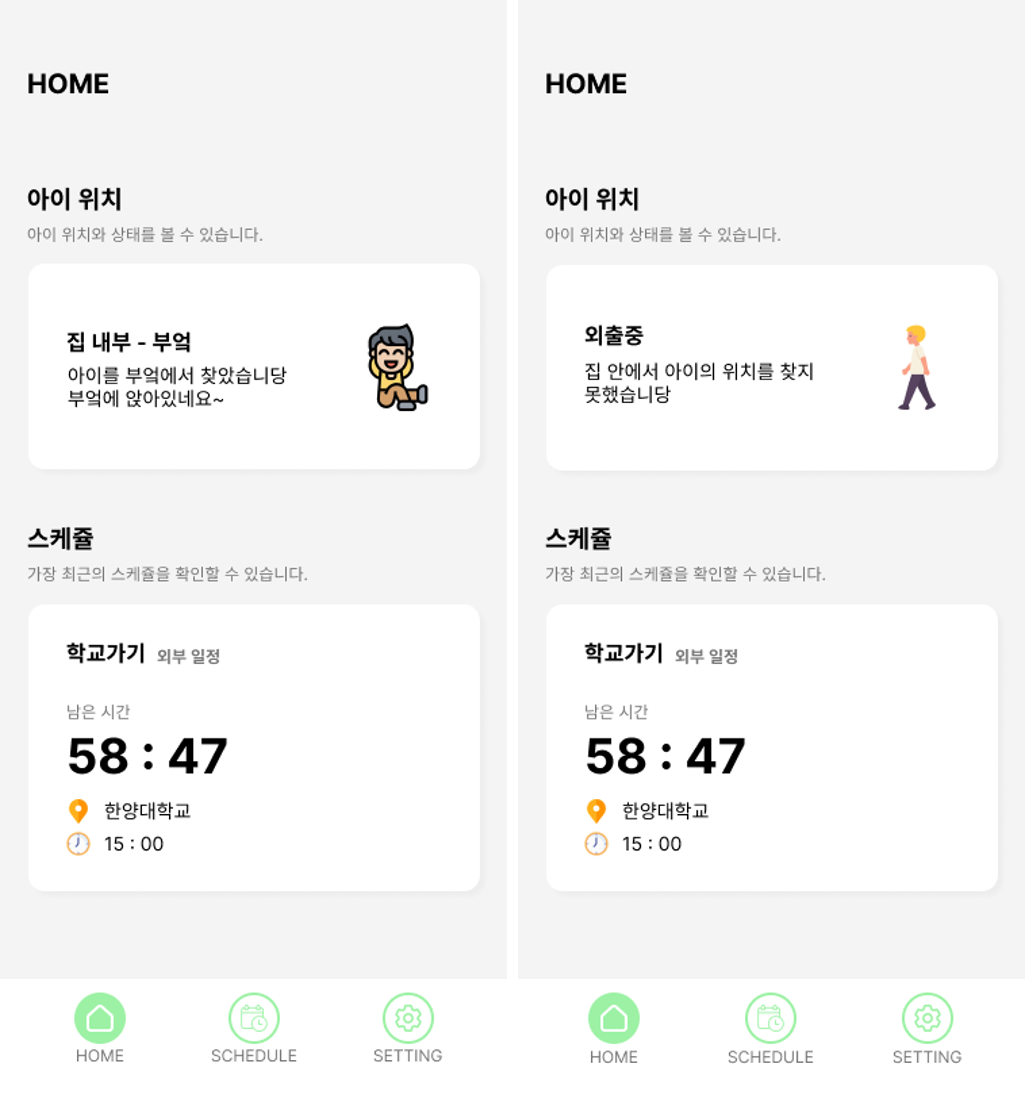
\includegraphics[scale=0.4]{images/main.png}\end{figure}  
    \begin{enumerate}[label=\alph*.]
        \item {\large{Kid's current status}} \\
        The kid’s current status block is located at the upper half of the page. It shows two statuses whether the kid is at home or not. \\
        \begin{enumerate}[label=\roman*.]
            \item {\large{IN: If he or she is at home, then the word ‘IN’ will be emphasized. Furthermore, it provides the location of the kid when the kid is in the house. For example, when the kid is in the living room, Under the IN/OUT icon, the location is shown as “living room” as a text.}} \\
            \item {\large{OUT: In the opposite case, the word ‘OUT’ will be highlighted. }} \\
        \end{enumerate}
        \item {\large{Kid’s schedule}} \\
        The kid’s schedule status block is located at the lower half of the page. This block is divided into three parts. \\
        \begin{enumerate}[label=\roman*.]
            \item {\large{The time remaining until the most immediate schedule}} \\
            The unit of time is minute until 59 minutes, and time over 60 minutes is shown as one hour. Minutes don’t count as an hour, for example, 16 minutes in 76 minutes, are discarded. So 76 minutes are shown as one hour.
            \item {\large{The place where the schedule is taken}}
            \item {\large{The starting time of the next event}}\\
        \end{enumerate}
        For example, let’s say the time is now 7’o clock and school begins at 8’o clock. Then the time remaining will be 60 minutes. \\
        Three things will be shown which are: \\
        \begin{enumerate}[label=\roman*.]
            \item {\large{60 minutes (Time remaining)}} 
            \item {\large{School (The place)}}
            \item {\large{08:00 (The starting time of the next event)}}\\
        \end{enumerate}  
        \item {\large{Footer}} \\
        \begin{figure}[H]\centering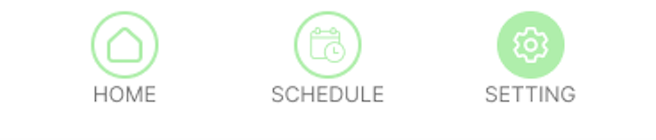
\includegraphics[scale=0.65]{images/footer.png}\end{figure} 
        In the footer, there are three buttons; home, schedule, and configuration. Home is the current status whereas the schedule is the button to move to the schedule managing page. Clicking the configuration button redirects to the configuration page. It is represented with a gear wheel icon. This page includes four blocks. \\
        \begin{figure}[H]\centering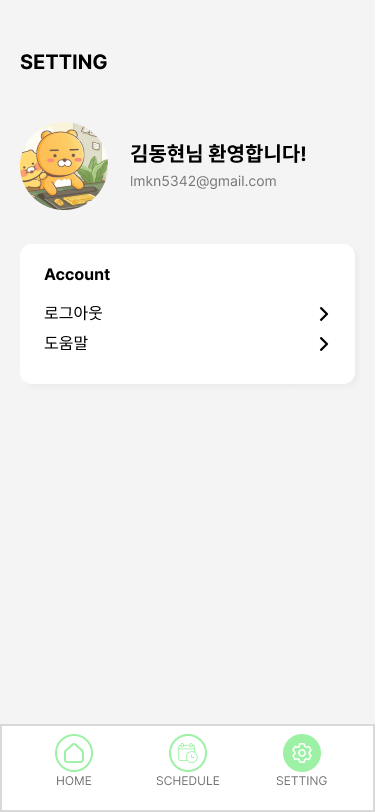
\includegraphics[scale=0.3]{images/setting.png}\end{figure}        
        \begin{enumerate}[label=\roman*.]
            \item {\large{Profile}} \\
            The text “Hello, “ + user\_name + “!” is written and right next to the exclamation mark, there is a random profile picture. If the user clicks the picture, a pop-up will occur. From 12 photos, the user can pick and use one. There will be an X button to close the pop-up.
            \item {\large{Setting}}\\
            The setting includes a few swipeable buttons. It includes version changes between kid mode and elderly mode, profile changes, and nickname changes. 
            \item {\large{Help}}\\
            This shows the tutorial of the page.
            \item {\large{Logout}}\\
            Represented with an open door icon, the footer has a logout function. \\
            \end{enumerate}            
    \end{enumerate}
    \item {\large{Schedule managing page}} \\
    This page is designed in order to display the kid’s schedule. Adding a schedule and deleting a schedule are the two most important functions on this page. This page includes the following: \\
    \begin{figure}[H]\centering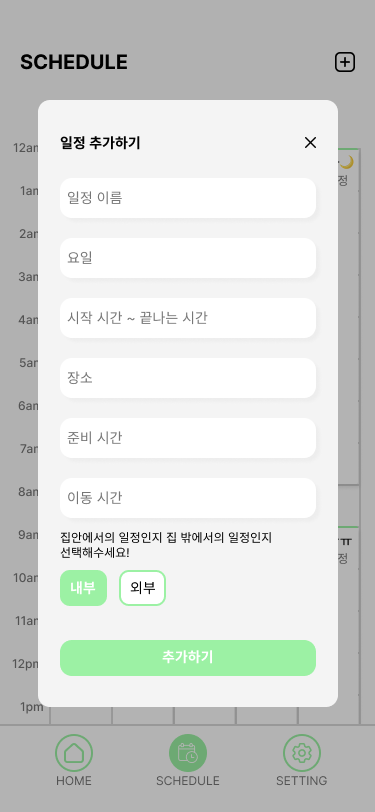
\includegraphics[scale=0.3]{images/add.png}\end{figure} 
    \begin{enumerate}[label=\alph*.]
        \item {\large{Schedule add button: This button is for adding a new schedule. This button uses a plus sign. If the user clicks the button, the schedule adds pop-up screen appears. the pop-up screen consists of six fields and three buttons.}} \\
        \begin{enumerate}[label=\roman*.]
            \item {\large{Field 1: Title of the schedule (string)}} 
            \item {\large{Field 2: Starting/end time of the schedule (string)}} 
            \item {\large{Field 3: Starting/end time of the schedule (timestamp)}} 
            \item {\large{Field 4: Location of the schedule (string)}} 
            \item {\large{Field 5: Time takes for preparation (string)}} 
            \item {\large{Field 6: Travel time (string) }}   
            \item {\large{Button 1, 2: Buttons to choose whether the location of the schedule is inside or outside the house}} 
            \item {\large{Button 3: Button named as “add” whose background color is gray when it’s deactivated, and colored when all 3 fields are fulfilled}} \\            
        \end{enumerate}
        \begin{figure}[H]\centering 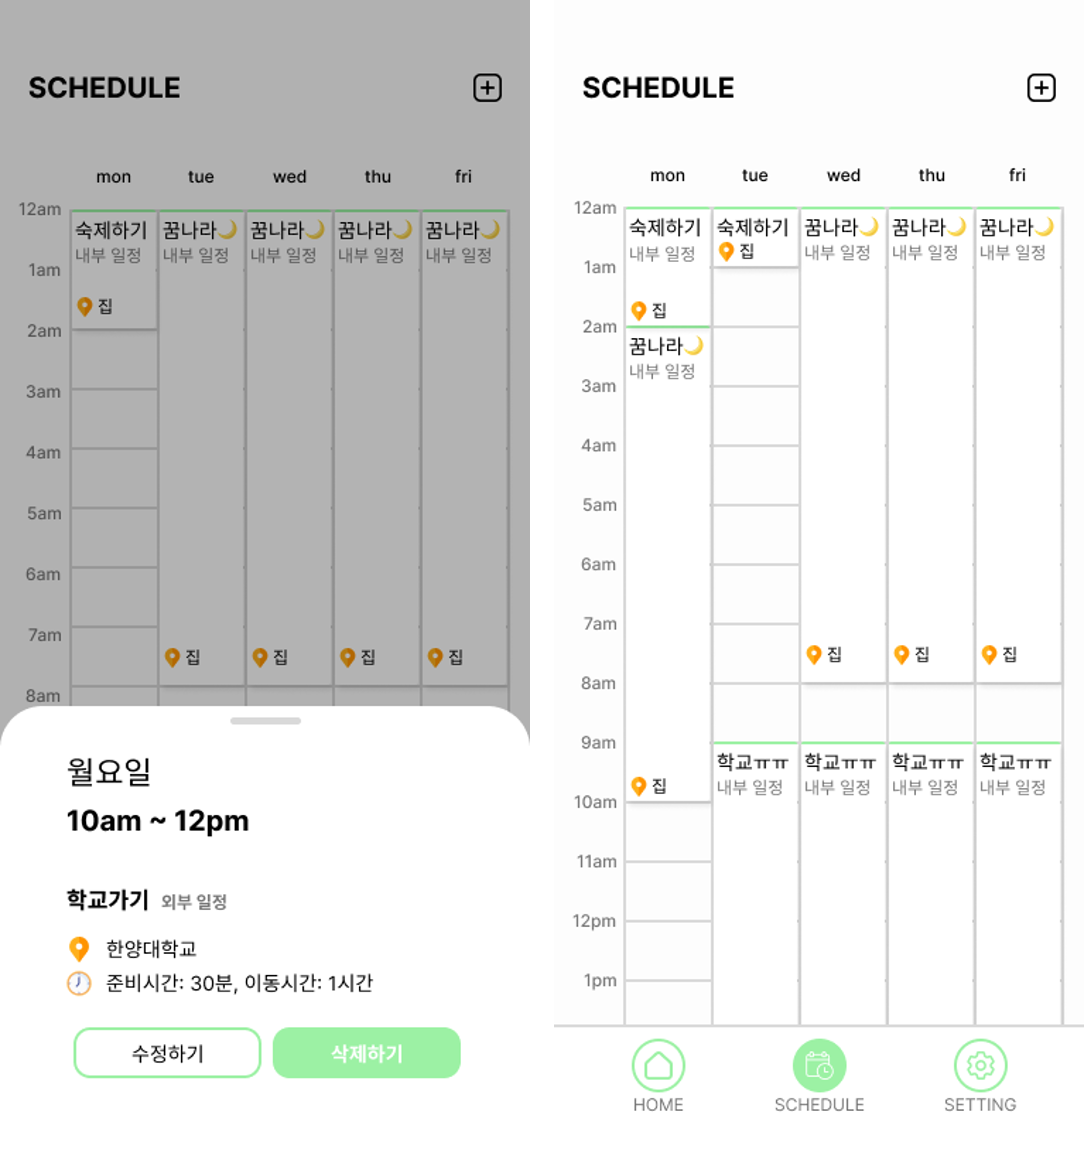
\includegraphics[scale=0.4]{images/schedule.png}\end{figure}        
        \item {\large{Schedule table: This table is located at the very center of the page. The table describes the overall outline of the kid’s schedule in form of a weekly timetable. Thus, it will be represented in row and column format. Its column represents every day of the week and the row represents the time, which is segmented into an hour per block. }} \\
        \begin{figure}[H]\centering 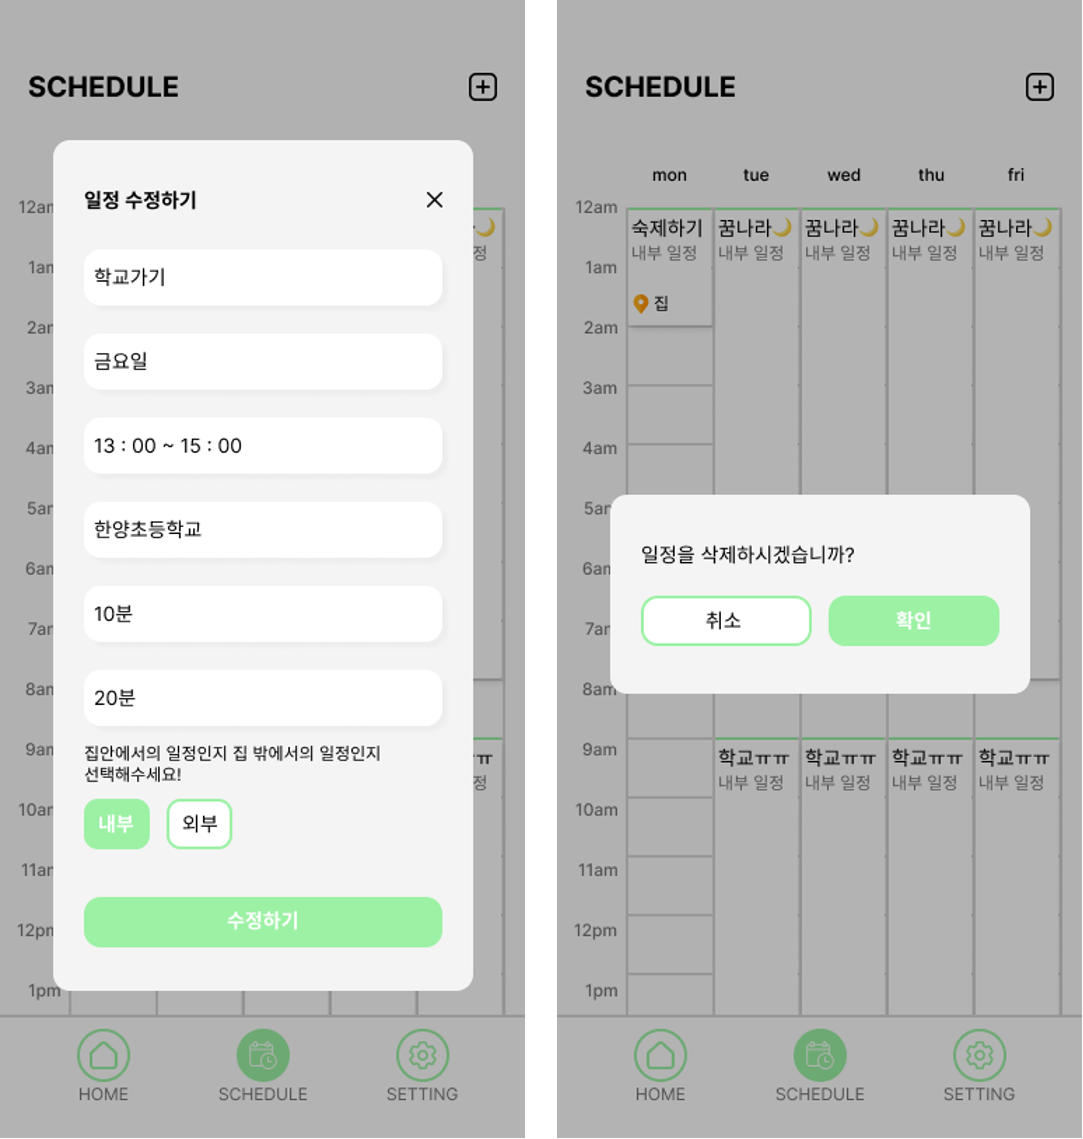
\includegraphics[scale=0.4]{images/modify.png}\end{figure} 
        \item {\large{Modify Schedule: When clicking the schedule, the bottom sheet menu pops up. It includes the date, starting time, finishing time, the title of the event, the location, and the two buttons; modify and delete. }} \\      
        \begin{enumerate}[label=\roman*.]
            \item {\large{Modify button: When clicking it, it leads to the modify pop-up. This is similar to the schedule add pop-up. The only difference is that the modified pop-up is already filled with the original schedule and has a different title. The user only has to change what he or she needs to change. }} \\
            \item {\large{Delete button: When clicking the Delete button, it asks if you really want to delete the schedule with a pop-up message. If the user clicks “cancel”, written in the gray box, the user return to the exiting pop-up. Or if the user clicks “delete”, written in Redbox, the schedule is ultimately deleted and the schedule table will no longer contain that schedule. }} \\
        \end{enumerate}
    \end{enumerate}
\begin{center}\large{Server-side}\end{center}
\begin{enumerate}[label=\arabic*.]
    \item {\large{Web server}} \\
    A web server consists of a single page with one button, the alarm stop button. Here is the step of how the button works. If the user clicks the button, the sound playing by the alarm stops. \\
    \item {\large{API server}} \\
    API server sends data needed for APP(Front\_end) and AI speaker response. API server has its own small database, called SQLite, which is utilized by Django and Django rest framework. SQLite contains these kinds of fields: \\
    \begin{enumerate}[label=\alph*.]
        \item {\large{String name}} \\
        It contains the names of children that which app is trying to keep track of. It is stored in the format of a string. It also enables distinguishing each and every child which leads to a personalized solution for the kid. \\
        \item {\large{Boolean is\_kid\_home}} \\
        There are two available states which are True and False. If the kid is at home, the vacuum cleaner will detect the child and will send the signal to the core(station) and after processing the signal, the result is applied to this variable. \\
        \item {\large{String where\_is\_kid}} \\
        Many states are available in this case. The robot vacuum cleaner will detect the child in a specific place( for ex. the living room, or the child's room). A range of places can be chosen by the parents. \\
        \item {\large{String is\_kid\_ready}} \\
        Home Alone divides the kid’s status briefly into three states. It is standing, sitting, and laying. 0 stands for standing. 1 stands for sitting. 2 stands for laying. If the schedule is upcoming, and if the motion detector detects the kid’s motion and sends 1 or 2 for this field, it refers that kid is not ready for its schedule. \\
        \item {\large{String schedule\_url}} \\
        Schedule\_url contains the directory path of the schedule’ file(JSON)s URL. There are two reasons for the existence of schedule\_url in SQLite. If all schedule data is saved in the SQLite, then there will be a security issue. There is a chance of information leakage. In addition, schedule data is too big to be put into the SQLite server. So we chose to make a separate file to save the schedule to avoid such problems. \\
        In schedule data(JSON file)of each time unit, it contains below fields: \\
        \begin{enumerate}[label=\roman*.]
            \item {\large{id: ID field contains the id of its schedule. For each schedule, it contains a unique id for a specific schedule. This, therefore, distinguishes the schedule from other schedules. Also, if a given time unit does not have a schedule, this field is kept at 0. }} \\
            \item {\large{title: Field containing the name of the schedule }} \\
            \item {\large{title: Field containing the name of the schedule }} \\
            \item {\large{location: Field containing where the schedule is held }} \\
            \item {\large{scheduleType: field containing whether the schedule is held inside or outside }} \\
            \item {\large{readyTime: field containing information of how much time it takes to prepare for its schedule }} \\
            \item {\large{movingTime: field containing information of how much time it takes to get to the location where the schedule is being held}} \\   
        \end{enumerate}
    \item {\large{String stage\_url}} \\
    A stage is a time unit that has been previously defined into 10 minutes. Our team has differentiated its stage into five states: \\
        \begin{enumerate}[label=\roman*.]
            \item {\large{not in home: a stage the kid should not be at the house }} \\
            \item {\large{No schedule: a stage where the kid is at home but he or she does not have to get ready for the next schedule }} \\
            \item {\large{Safety\_Margin: a stage that it is desirable for the kid to be ready for the next schedule compared with schedule data }} \\
            \item {\large{Need to Ready: regarding the schedule data field “ready time”, which the user has previously entered in case of expecting to be ready for a specified schedule, it is a stage that the kid should start preparing. }} \\
            \item {\large{Move: regarding the schedule data field “Moving Time”, which the user has previously entered, it is a stage where the kid should not be home. }} \\
        \end{enumerate}
    Also, API server responds to various requests from an App(Frontend):\\
        \begin{enumerate}[label=\roman*.]
            \item {\large{Get Kids status }}\\
            When the app requests the kid’s status, the API server returns in JSON format containing the field of is\_kid\_home and where\_is\_kid, by referring to its SQLlite DB. \\
            \item {\large{Get init\_schedule all }} \\
            When the app requests initial total schedule data, the API server opens the JSON file, by referring to its schedule\_url. And then it returns all data to the app in JSON format. \\
            \item {\large{Get recent schedule }} \\
            After requesting total schedule data, the API server opens the JSON file using schedule\_url. And then it returns the partial schedule data in a one-time slot, that is ten minutes, to the app in JSON format.
            \item {\large{Delete schedule }} \\
            This request is held when the user tries to delete a certain user’s schedule. The app will send time unit information to the API server. And the API server will parse from that information and delete it from the corresponding time unit. And the API server will give a response, the success message to the app. \\
            \item {\large{Add Schedule }} \\
            When the user tries to add a schedule to schedule data, this method is used. The app will send the schedule’s id, title, and time containing day, startHour, endHour, endMin, schedule Type, location, readytime, and movingtime. \\
            Then the API server will parse data by using the time field and put the corresponding values of the time field into schedule data. If there is no previous schedule in the certain time field, the schedule should be added to the schedule file. Then the success message is sent to the app. However, if there is a schedule in the selected time unit, the schedule will not be added and the user will receive the fail message. \\
            \item {\large{Schedule Modify }} \\
            This request is held when the user tries to modify the user’s schedule. Modify includes the concept of delete and add. When the app sends information about a certain schedule, the API server will parse data by using fields of prevTime and Time. By using the prevTime field, the API server will delete the corresponding existing schedule. By using the Time field, the API server will add the corresponding schedule to JSON file. And if delete and add are both satisfied, the API server sends a success message to the app. Otherwise, it will return a fail message. \\
            \item {\large{Current time schedule }} \\
            This request searches the most recent upcoming schedule of the user. API Server will get the current time from the date time module, and get data about its upcoming schedule by searching the algorithm. There are three cases for searching its upcoming schedule. First, if the next upcoming time unit`s schedule is empty, which is divided by 10 minutes, the program searches the upcoming next schedule and returns its start time and end time. Second, if the next upcoming time unit`s schedule is not empty, the searching algorithm has to decide whether this schedule was in progress in the past or not. If the case was the former, the user has to find the next upcoming schedule. Else, the user can recognize that the upcoming time unit is the start time of the next schedule. API server will return App with schedule information, providing starttime and endtime in JSON format. \\
        \end{enumerate}
    \end{enumerate}
    \item {\large{Station}} \\
    \begin{enumerate}[label=\alph*.]
        \item {\large{Core}} \\
        The Core is executed every 10 minutes. It should have the functions written below: \\
        \begin{enumerate}[label=\roman*.]
            \item {\large{It reads converted stage data.}}
            \item {\large{It updates the stage in the DB for saving the current stage. So, the stage manager should include a function that enables transactions with the database.}}
            \item {\large{It executes state manager. The specific explanation of the state manager is written below. }} \\ 
        \end{enumerate}
        \item {\large{Core should have following variables: }} \\
        \begin{enumerate}[label=\roman*.]
            \item {\large{String current\_stage (from DB)}}
            \item {\large{String next\_stage}}\\
        \end{enumerate}
        \item {\large{State manager (executed by stage manager)}} \\
        \begin{enumerate}[label=\roman*.]
            \item {\large{The state manager should have the following functions: }}
            \begin{itemize}
                \item {With 3 global variables (Is\_kid\_home, Where\_is\_kid, Is\_kid\_ready), the state manager decides which state should the station be.}
                \item {Update state in DB data for saving current state }
                \item {execute: There are two functions inside the 'execute'. First is the robot cleaner's direction. It sends directions to the robot cleaner. This direction should make the robot cleaner to be in observing mode. The second is the SMS module. It sends an SMS message to parents or supervisors with (주)알리는 사람들 API. } \\
            \end{itemize}
            \item {\large{stage manager should have following variables: }}
             \begin{itemize}
                \item {String current\_state (from DB)}
                \item {String next\_state}
                \item {Boolean Is\_kid\_home}
                \item {String Where\_is\_kid}
                \item {String Is\_kid\_ready} \\     
            \end{itemize}
        \end{enumerate}
        \item {\large{Schedule data manager}} \\
        \begin{enumerate}[label=\roman*.]
            \item {\large{Convert schedule(JSON) given by app to stage data(JSON)}} 
            \item {\large{Converter utilizes following rule for interpreting schedule into stage}} 
            \item {\large{If the user modifies the schedule locally in APP, this module applies that change to JSON data in the URI saved in DB.}} \\
        \end{enumerate}
    \end{enumerate}      
    \item {\large{DB}} \\
    DB consists of the following fields: \\
    \begin{enumerate}[label=\alph*.]
        \item {\large{upon single userid}} 
        \item {\large{schedule\_uri: field for saving schedule\_JSON data}} 
        \item {\large{stage\_uri: field for saving stage\_JSON data}} 
        \item {\large{Boolean Is\_kid\_home: The available state is true or false.}} 
        \item {\large{Str Where\_is\_kid: The available state is kid\_room, living\_room, kitchen and etc. }} 
        \item {\large{Str Is\_kid\_ready: The available state is standing, sitting, and laying. }}
        \item {\large{Str current\_stage: field for saving and sharing current stage between functions}}
        \item {\large{Str current\_state: field for saving and sharing current state between functions}}
        \item {\large{int lazy\_cnt: field to be utilized for state manager implementation}}
        \item {\large{int alert\_cnt: field to be utilized for state manager implementation}}
        \item {\large{int stage\_rep: field to be utilized for state manager implementation}} \\   
    \end{enumerate}
\end{enumerate}
\newpage

\section{\Large{Architecture design \& Implementation}}
\begin{enumerate}[label=\arabic*.]
    \item {\large{Overall Architecture}} \\
    \begin{figure}[H]\centering 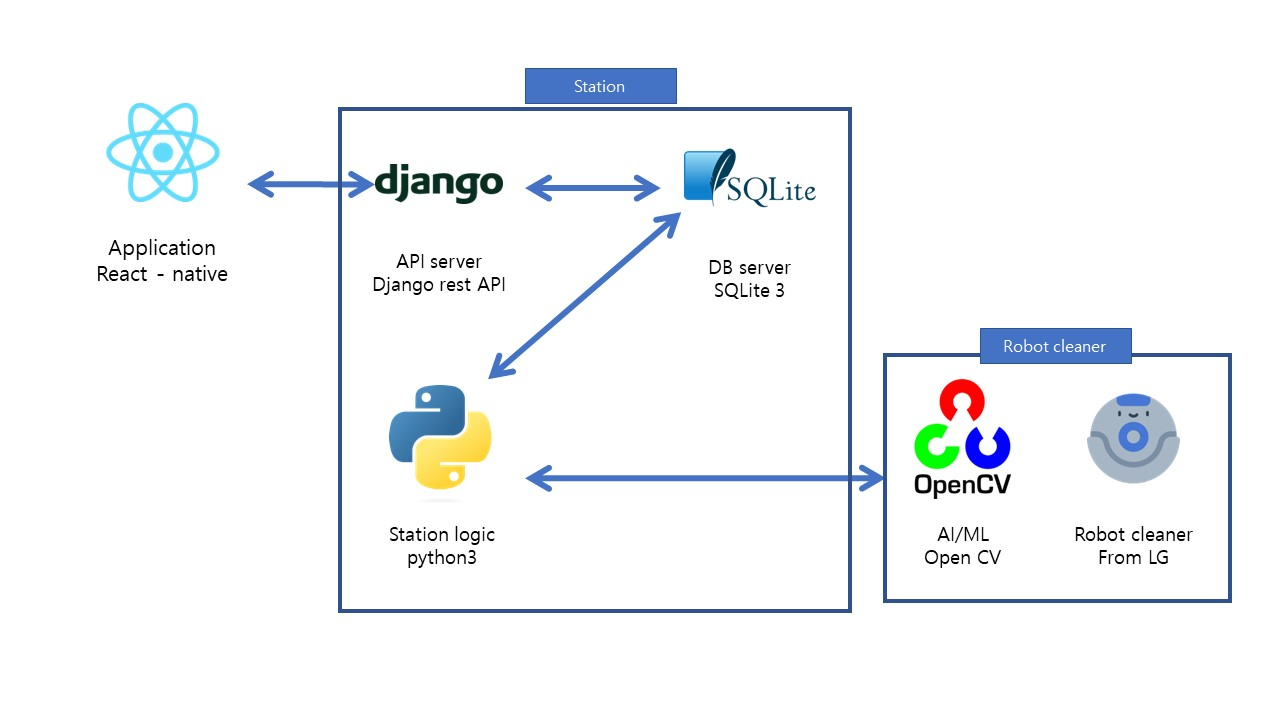
\includegraphics[scale=0.3]{images/overall_diagram.jpg}\end{figure} 
    \item {\large{Directory Organization}} \\
    \begin{enumerate}[label=\alph*.]
        \item {\large{Front end}}\\
        
        \tablefirsthead{\toprule Directory & File name \\}
        \tablehead{\toprule Directory & File name \\}
        \tabletail{\midrule}
        \tablelasttail{\bottomrule}
        \begin{supertabular}{p{0.5\linewidth} | p{0.3\linewidth} p{0.05\linewidth}}
        \midrule
        /components/atoms & \makecell[l]{.Avatar.js\\.Box.js\\.Card.js\\.Container.js\\.Icon.js\\.Input.js\\.Picker.js\\.Text.js\\.TimePicker.js} \\
        \midrule
        /components/molecules & \makecell[l]{.BottomNavigationBar\\.Item.js\\.Button.js\\.DailyScheduleMatrix.js\\.Menu.js\\.ProfileBox.js\\.ScheduleBox.js\\.TextWithIcon.js} \\
        \midrule
        /components/organisms & \makecell[l]{.BottomNavigationBar.js\\.BottomSheet.js\\.Header.js} \\
        \midrule
        /hooks & \makecell[l]
        {.useDidMountEffect.js\\.useFade.js\\.useTimer.js} \\
        \midrule
        /modal/basic & \makecell[l]
        {.BasicModalContainer.js\\.BasicModalPresenter.js} \\
        \midrule
        /modal/schedule & \makecell[l]
        {.ScheduleModalContainer.js\\.ScheduleModalPresenter.js} \\
        \midrule
        /navigators & \makecell[l]
        {.BottomNavigator.js\\.Navigator.js} \\  
        \midrule
        /pages/home & \makecell[l]
        {.HomeContainer.js\\.HomePresenter.js} \\
        \midrule
        /pages/login & \makecell[l]
        {.LoginContainer.js\\.LoginPresenter.js} \\
        \midrule
        /pages/schedule & \makecell[l]
        {.ScheduleContainer.js\\.SchedulePresenter.js} \\    
        \midrule
        /pages/setting & \makecell[l]
        {.SettingContainer.js\\.SettingPresenter.js} \\
        \midrule
        /redux & \makecell[l]
        {.rootReducer.js\\.store.js} \\
        \midrule
        /redux/reducers & \makecell[l]
        {.Input.js\\.UserData.js} \\
        \midrule
        /sheet	& .BottomSheet.js \\
        \midrule
        /sheet/scheduleSheet & \makecell[l]
        {.ScheduleSheetContainer.js\\.ScheduleSheetPresenter.js} \\
        \midrule
        /utils & \makecell[l]
        {.Auth.js\\.createSnackbar.js\\.string.js} \\
        \midrule
        /	& .App.js \\
        \end{supertabular}  
        \newpage
        \item {\large{Back end - Station}}\\
        
        \tablefirsthead{\toprule Directory & File name \\}
        \tablehead{\toprule Directory & File name \\}
        \tabletail{\midrule}
        \tablelasttail{\bottomrule}
        \begin{supertabular}{p{0.5\linewidth} | p{0.3\linewidth} p{0.05\linewidth}}
        \midrule
        /Homealone\_station & \makecell[l]{.Core.py\\.state\_manager.py\\.DB\_fetch.py\\.DB\_mod.py\\.DB\_reset.py\\.remote\_control.py\\.sms\_function.py\\stationdb.sqlite3}\\
        \midrule
        /Homealone\_station/ schedule\_JSON & \makecell[l]
        {.ScheduleData.json}\\
        \midrule
        /Homealone\_station/ schedule\_JSON & \makecell[l]
        {.stage\_1.json}\\
        \end{supertabular}   
        \newline
        \newline
        \item {\large{Back end - API}}\\ 
        
        \tablefirsthead{\toprule Directory & File name \\}
        \tablehead{\toprule Directory & File name \\}
        \tabletail{\midrule}
        \tablelasttail{\bottomrule}
        \begin{supertabular}{p{0.5\linewidth} | p{0.3\linewidth} p{0.05\linewidth}}
        \midrule
        /homealone\_api/ api\_se & \makecell[l]
        {.\_init.py\\.asgi.py\\.settings.py\\.wsgi.py\\.urls.py}\\
        \midrule
        /homealone\_api/ my\_api & \makecell[l]  {.\_init.py\\.admin.py\\.apps.py\\.tests.py\\.models.py\\.serializers.py\\.urls.py\\.views.py}\\
        \midrule
        /homealone\_api & \makecell[l]
        {.db.sqlite3\\.manage.py}\\
        \end{supertabular}
    \end{enumerate}
    \newpage
    \item {\large{Module 1: front end}} \\
    \begin{enumerate}[label=\alph*.]
        \item {\large{Purpose}}\\
        It is used to provide visible services to users. The application is built through this process. It allows parents or supervisors to keep an eye on the kid every time everywhere through HomeAlone. \\
        \item {\large{Functionality}}\\
        It largely provides two functions; schedule management and checking child status. Front-end gets the schedule data from the server, converts it to the appropriate type, and sets the timer. It also has a local database that can store user schedule IDs for schedule addition. And it takes the child's status data from the server and renders it in a form that users can easily understand.\\
        Due to the linkage of the Firebase and the client, the management of users can be easily done. The user can log in using Firebase Google Earth. When logging in, the UID has been automatically created as well as a user board. \\
        \item{\large{Location of Source Code}}\\
        /homealone\_integrate/homealone\_client\\
        \item Module explanation\\
        \begin{enumerate}[label=\roman*.]
            \item {\large{Login logic}}\\
            A login function is implemented using Firebase, including Google login, Apple login, and Facebook login. An instance was created by the setting provider in order to use the Google login function among them. By using the Google provider instance, it redirects to the Google login page and asks the user to log in with the Google account. \\
            When login through firebase is detected, user information is shared globally and the page is moved to the main screen. Redux technology was used to share user information in the global variable. Previously, when transmitting certain data to the next screen, the value had to be handed over as a component parameter. However, with redux, the data can be put in storage and taken out, and written from any screen. When displaying user information on the setting page, the user information was saved using redux and was used. \\
            Since it takes a while to send authentication tokens and receive user information during the login process, if the screen stays still, the user may mistake it as lagging. Therefore, the login process is asynchronously processed, and progress animation is shown during login to provide a better user experience. \\
            \item {\large{Schedule page}}\\
            When the schedule page is first rendered, schedule data is received from the server. Axios, a promise-based HTTP client, was used to perform asynchronous processing. When the schedule data is successfully received, the data state is updated. Each time the data state is updated, a setScheduleData function is executed. This function processes the schedule json received from the server to render the schedule box. \\
            In Schedule json, 24 hours are divided into 10 minutes to store each schedule. While circulating schedule json through the loop, it counts how many schedules have the same id. For example, if there is a schedule with an id of 1 from 3:00 to 5:00 and an id of 2 from 6:00 to 7:00, json is processed in the form of {id: 1, count: 12}, {id: 0, count: 6}, {id: 2, count: 6}. \\
            It updates the schedule data state when the data processing is completed. When the state is updated, the schedule box starts to render. The height of the schedule box is dynamically set according to the count of the schedule. If the id of the schedule is 0, meaning that there is no schedule, a view with the height of the count is created. Otherwise, if the id is not 0, a scheduleBox component with the height of the count is created. \\
            \item {\large{Specific schedule}}\\
            The openSheet function is run when the schedule box is clicked. This function updates the state of the sheetVisable to render the bottom sheet. The schedule data and openDialog functions are handed over as parameters of the bottom sheet component to show detailed data of the schedule and to open a pop-up window where the user can delete or modify the schedule. \\
            When creating the openDialog function, useCallback hook was used. In general, when a function is created and handed over as a component's parameter, the function is regenerated every time it is rendered, which adversely affects performance. By creating a function using the useCallback hook, the function was optimized by allowing it to be reused. \\ 
            When rendering the bottom sheet, the react portal was used. React portal is a function that renders components outside the dependent DOM tree to another external DOM. If rendering is done on the current page, the bottom sheet is not rendered to the desired location because the current page exists on the bottom bar. Therefore, the component was rendered as a previous DOM without bottom bar using the react portal. \\
            \item {\large{Schedule modification}}\\
            The schedule modification pop-up window contains data of the current schedule in each input field in the schedule addition pop-up window. Hence, when the schedule data was transferred to the parameter, the value of the input field was set to distinguish between schedule addition and schedule modification. \\
            When pressing the Add Schedule button, the createSchedule function is run. As soon as it is executed, it first checks whether each input field is empty. If empty, a message such as "Please enter a schedule name!" is printed on the app screen and exits the function. It generates a schedule ID when all fields are filled in. The method of generating the schedule ID is as follows. Extract the id from the local database within the app. If ID does not exist, it returns 0. Then add 1 to the ID that is taken out to create a new schedule ID. The new ID is saved back to the local database. By storing the value in the local database, the value does not disappear even if the app is terminated, so the ID can be kept unique. \\
            When ID creation is completed, an API that adds the schedule is requested. When an API response arrives, the getScheduleData function is called. GetScheduleData is a function that receives schedule data from the server on the 2. Schedule page. By calling this function, the entire schedule data with the new schedule added is rendered on the screen. \\
            Pressing the Modify Schedule button calls the editSchedule function. This function consists of the same logic, except for the logic of generating an ID in the createSchedule function. \\
            \item {\large{Home page}}\\
            When the home page is rendered, the getKidStatus, getCurrentSchedule function is executed. When the getKidStatus function is executed, the current state of the child is retrieved from the server. Then it renders the UI by updating the state of kidStatus. \\
            When the getCurrentSchedule function is executed, the most recent schedule data is retrieved from the server. If the schedule data is successfully imported, the setTimer function is executed. The setTimer function calculates the time remaining until the latest schedule and updates the hours, minutes, and seconds states. \\
            Each time the hours, minutes, and seconds states are updated, the timer is set. Using the setInterval function, the second 1 is reduced every second. And when seconds, minutes, and hours all become 0, the timer is terminated using the clearInterval function. If there is no 0, the timer is performed by manipulating seconds, minutes, and hours in some cases. \\
        \end{enumerate}
    \end{enumerate}
    \item {\large{Module 2: back end}} \\ 
    \begin{figure}[H]\centering 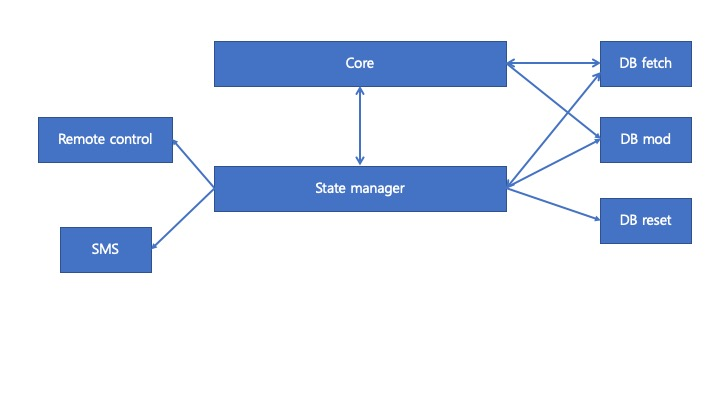
\includegraphics[scale=0.3]{images/flowchart.jpeg}\end{figure} 
    \begin{center}\large{Core module}\end{center} 
    \begin{enumerate}[label=\alph*.]
        \item {\large{Purpose}}\\
        There are three reasons for the station implementation. First, modeling DB’s current stage as the stage that brought from stage.json is done by the station server. Second, it decides whether the current stage is the same or not with the next stage. Third, it executes the state manager.\\
        \item {\large{Functionality}}\\
        A core module is executed every 10 minutes by apscheduler. Every 10 minutes, the following functions are executed. Core brings the current stage from DB and the next stage from stage.json. After comparing both, there are two branches. First, if they are not the same, meaning if the next stage is changed, the core executes the DB\_reset function. This resets values to the default value and executes state\_manager. Second, if they are the same, the state\_manager is executed. \\
        There are five steps to get stage from json file. 
        \begin{enumerate}[label=\roman*.]
            \item {\large{Using datetime.datetime.now, bring current time from local}}
            \item {\large{With that time, create timestamp with ts\_h(hour), ts\_m(minute)l}}
            \item {\large{Connect sqlite3 file and fetch stage\_uri data (location of stage.json)}}
            \item {\large{Get matching stage data from json file using timestamp and stage\_uri}}
            \item {\large{return\ current\_stage (brought from json)}}\\
        \end{enumerate}
        \item{\large{Location of Source Code}}\\
        \large{/homealone\_integrate/homealone\_station/Core.py}\\   
        \item {\large{Used library}}
        \begin{enumerate}[label=\roman*.]
            \item {\large{time: For delaying execution of codes}}
            \item {\large{JSON: To open JSON file}}
            \item {\large{date time: To fetch current time from local time}}
            \item {\large{SQLite3 : To access DB data}}
            \item {\large{apschduler: To execute this Core every 10 minutes}}
        \end{enumerate}
    \end{enumerate}
    \begin{center}\large{State manager module}\end{center} 
    \begin{enumerate}[label=\alph*.]
        \item {\large{Purpose}}\\
        The state manager module reacts to the stage which is decided by Core. This is done by deciding the state with two variables; is\_kid\_home and  is\_kid\_ready.\\
        \item {\large{Functionality}}\\
        The module gets the current stage every 10 minutes and based on the stage, the following functions are executed. It also brings the current stage from DB and finds a matching stage from the stage list. If the matching stage is found, the current state is decided by following the rule in the following table.\\
        \begin{figure}[H]\centering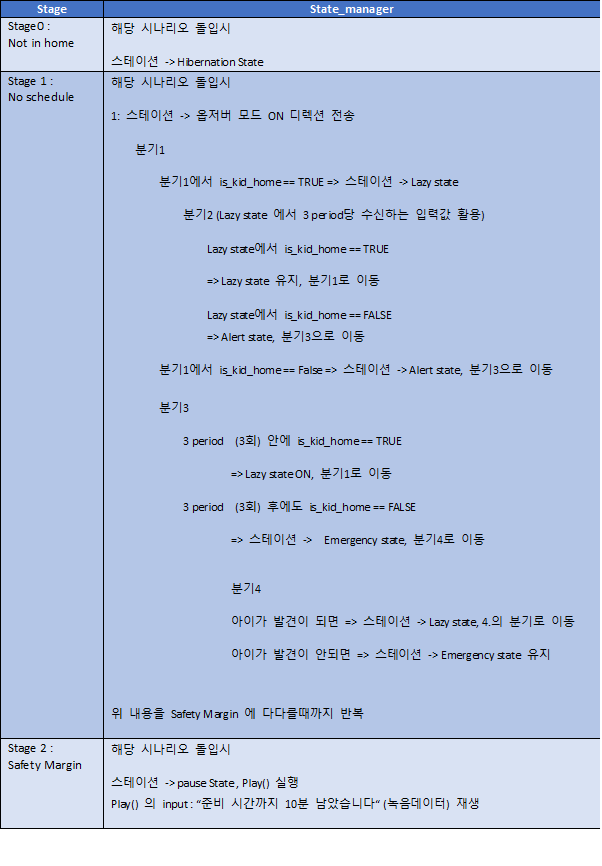
\includegraphics[scale=0.35]{images/rule1.png}\end{figure}
        \begin{figure}[H]\centering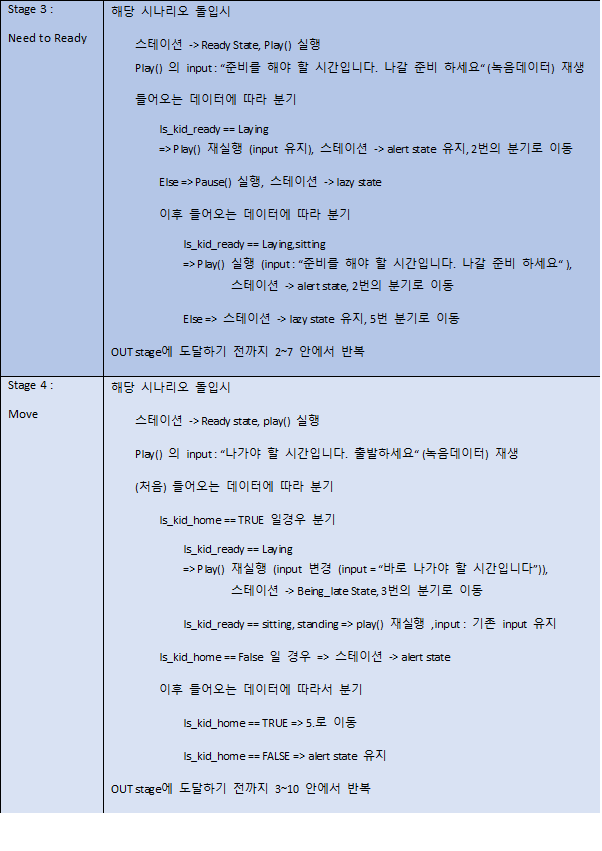
\includegraphics[scale=0.35]{images/rule2.png}\end{figure}
        Execute reaction for each state like following rules.
        \begin{figure}[H]\centering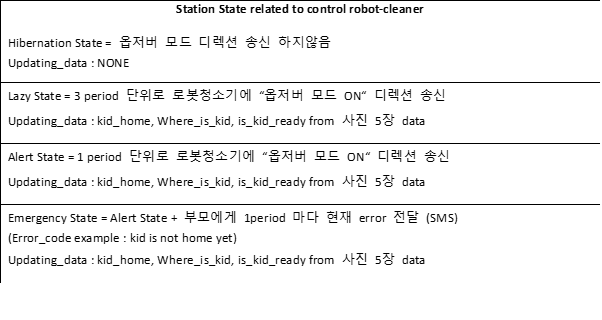
\includegraphics[scale=0.35]{images/rule3.png}\end{figure}
        \item {\large{Location of Source Code}}\\
        ./homealone\_station/ state\_manager.py \\
        \item {\large{Used library}} 
        \begin{enumerate}[label=\roman*.]
            \item {\large{time: For delaying execution of codes }}
            \item {\large{JSON: To open JSON file }}
            \item {\large{date time: To fetch current time from local time }}
            \item {\large{SQLite3: To access DB data}}
        \end{enumerate}
    \end{enumerate}
    \begin{center}\large{DB fetch module}\end{center} 
    \begin{enumerate}[label=\alph*.]
        \item {\large{Purpose}}\\
        DB fetch module simplifies the fetching mechanism on DB and makes code as a library for multiple uses. \\
        \item {\large{Functionality}}\\
        Each function in module follows naming rule: ‘get\_’+(field\_name).
        \item {\large{Location of Source Code}}\\
        ./Homealone\_station/DB\_fetch.py \\
        \item {\large{Used library}} \\
        SQLite: To access DB data
    \end{enumerate}  
    \begin{center}\large{DB mod module}\end{center} 
    \begin{enumerate}[label=\alph*.]
        \item {\large{Purpose}}\\
        This module simplifies modeling mechanism on DB and makes code as library for multiple use. \\
        \item {\large{Functionality}}\\
        Each function in module follows naming rule: 'set\_' + (field\_name). \\
        \item {\large{Location of Source Code}}\\
        /Homealone\_station/DB\_mod.py\\
        \item {\large{Used library}} \\
        SQLite: To access DB data
    \end{enumerate}
    \begin{center}\large{DB reset module}\end{center} 
    \begin{enumerate}[label=\alph*.]
        \item {\large{Purpose }}\\
        DB reset module simplifies resetting mechanism on DB and makes code as library for multiple use.\\
        \item {\large{Functionality }}\\
        Each function in  module follows naming rule: 'reset\_' + (field\_name). Therefore, this module resets data on DB.\\
        \item {\large{Location of Source Code}}\\
        ./Homealone\_station/DB\_reset.py\\
        \item {\large{Used library}} \\
        SQLite: To access DB data
    \end{enumerate}  
    \begin{center}\large{SMS module}\end{center} 
    \begin{enumerate}[label=\alph*.]
        \item {\large{Purpose}}\\
        This module creates library for sending SMS to simplify sending process. \\
        \item {\large{Functionality}}\\
        First, get message to be sent as a argument and add the message into actual payload with pre-written payload (mostly credential data). Try sending message to 알리고 server (run by (주)알리는 사람들, SMS API server), and receive response from 알리고 server.\\
        If, result code is not 1 (not 1 == unsuccessful request), print alert message.\\
        Else, no message appears. If exceptions happen, print alert message.\\
        \item {\large{Location of Source Code}}\\
        ./Homealone\_station/DB\_reset.py\\
        \item {\large{Used library}} \\
        request: to send HTTP request to 알리고 server \\
    \end{enumerate}  
    \item {\large{Module 3: API Server}} \\
    \begin{enumerate}[label=\alph*.]
        \item{\large{Purpose}}\\
        API server is a path between APP(front-end) and Station server(main database).  The station server updates kids' status in a predefined time unit(10 minutes). Thus, the app should have access to real-time updated status. Also, the front-end needs to get schedule data from the Linux server. In order to get and update inputs and outputs, definitely path is needed.\\
        \item{\large{Functionality}}\\
        The API server mainly provides responses that the front-end needs, by using methods of CRUD(Create, Read, Update, Delete) that API REST basically provides. It can also retrieve data from its own server called SQLite. When the app recalls its kids' status or current schedule by using a searching algorithm, it can therefore function as parsing data. Lastly, when the station server tries to update kid’s information, the API server becomes a coordinator between two agents; app and core server. It serves as a temporary database in order to convey the required information that the app needs.\\
        \item{\large{Location of Source Code}}\\
        /homealone\_integrate/homeAlone\_API\\
        \item{\large{Class Component}}\\
        \begin{enumerate}[label=\roman*.]
            \item{\large{api\_se/settings.py}}\\
            This file is constructed for setting up Django for projects. It contains a database field to set a temporary database called SQLite. Also, it sets server time automatically for purpose of internationalization. \\
            \item{\large{my\_api/models.py}}\\
            It is a file responsible for making tables in the SQLite database automatically. It contains two initial models, which are the Kid class and the Schedule class. They are in the format of classes. In the Kid class, the class contains id, name, is\_kid\_home, where\_is\_kid, schedule\_uri, and stage\_uri. It shares fields with the station server so that it can communicate directly with the station server. Also Schedule class contains the field of schedule\_dt in JSON field to serialize JSON data. \\
            \item{\large{my\_api/serializer.py}}\\
            This file helps to return corresponding fields which models created. This serializing process is used when user requests kid status. Front-end requests its method of get. This refers that the front-end needs all the values that class Kid has. Serializing is a must to perform this process. \\ 
            \item{\large{my\_api/views.py}}\\
            This file is responsible for the core functions of the API server. It deals with the request that the front-end made. The following response is done by the ‘view’ in the Django framework. There are two ways to make a view; class-based view, and function-based view. \\
            When the class-based view is generated, its CRUD response is made simultaneously and returns all the values in a specific view set. This is used when the app requests the kid's information. \\
            On the other hand, the function-based view is used when the front-end requests a certain field in SQLite or when it requests another action other than getting information inside the SQLite server. To get or modify schedule information, the API server has to access the schedule URI. Then it has to modify and get schedule data from that file. Therefore, returning its field to the SQLite server is not necessary for this process. \\
            Hence, views.py is responsible for parsing data in schedule data because the front-end needs modified JSON data. This task is done by the API server. \\
            \item{\large{my\_api/urls.py}}\\
            This file is used in creating URLs for each corresponding request from the app. By using view sets, the register method is a way to put all the related CRUD methods together about the specific models. Also, URLs are put separately to URL patterns to set URLs in function-based view.\\
        \end{enumerate}
        \begin{figure}[H]\centering 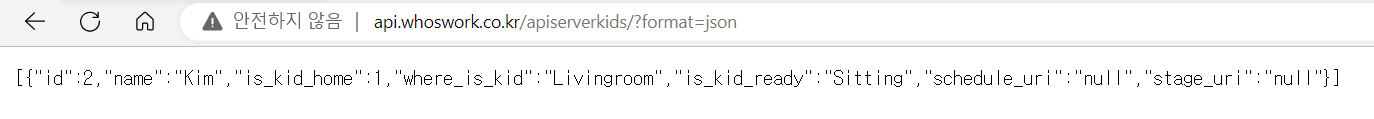
\includegraphics[scale=0.2]{images/api1.png}\end{figure} 
        Example of API request generated by urls.py- in order to get kid info \\
        \begin{figure}[H]\centering 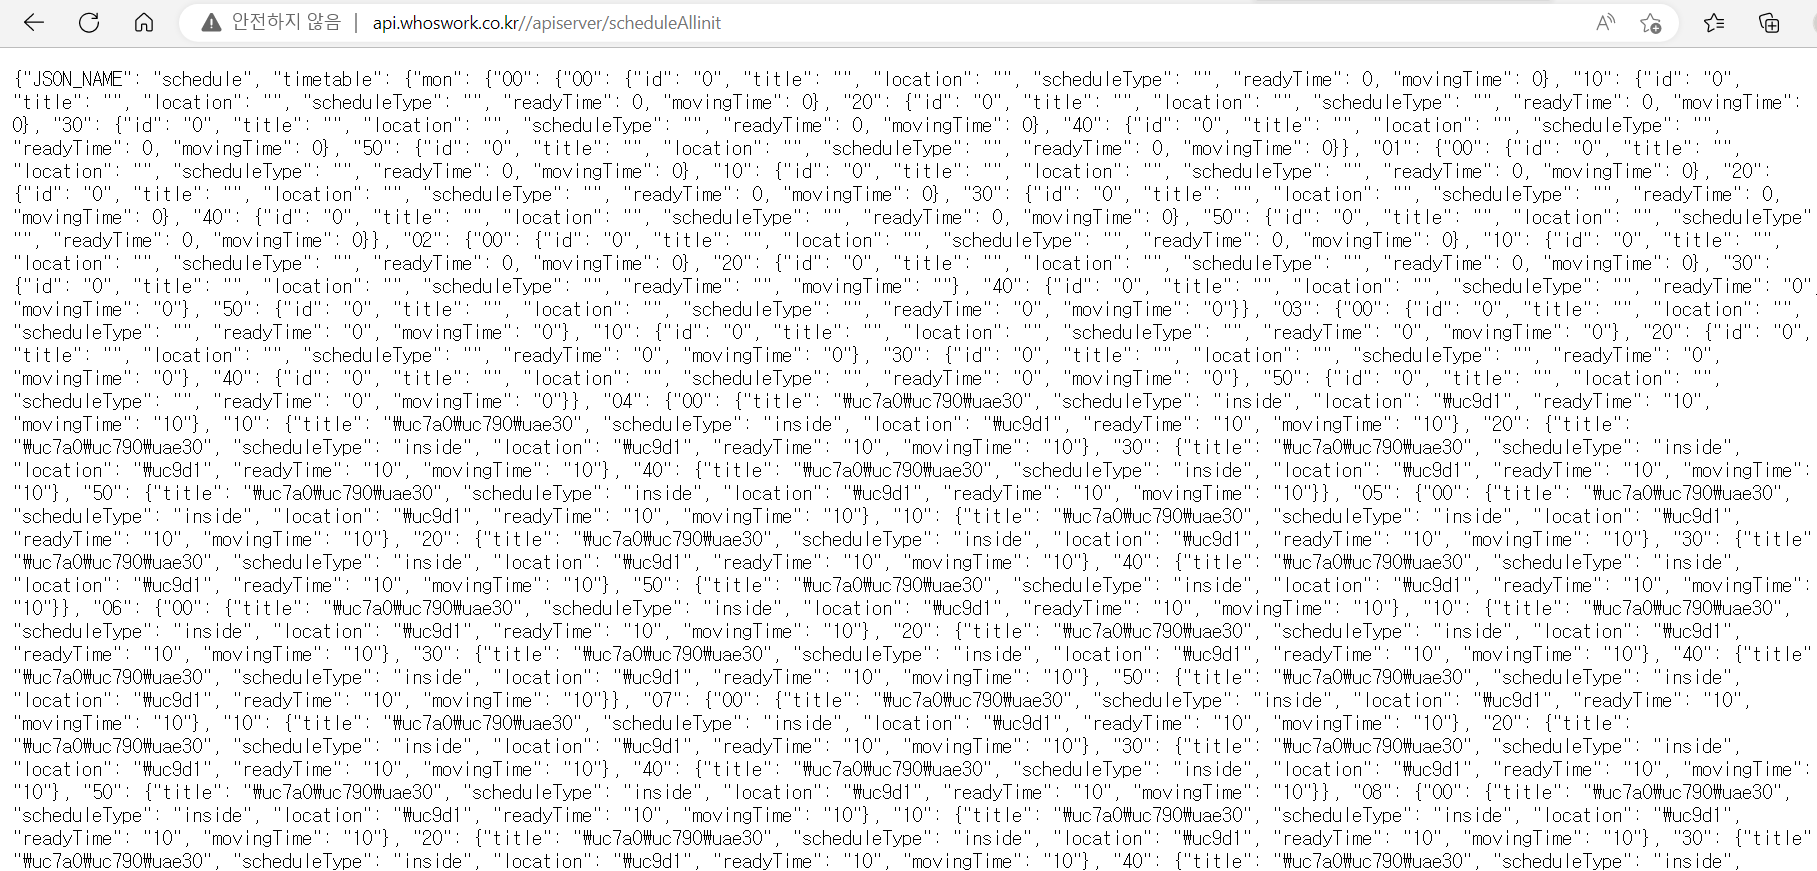
\includegraphics[scale=0.15]{images/api2.png}\end{figure} 
        Example of API request generated by urls.py- Get schedule all\_init \\
        \item{\large{Where it is taken from}}\\
        In terms of data, the requested information is conveyed in the body by front end, and the API server refers to the schedule data by schedule uri in SQLite field. \\
        \item{\large{How and why we used it}}\\
        Django was used in the API server for two reasons. First, in order to synchronize with the station server that is also built in Django, the API server used Django as well. This led to the convenience of the collaboration. Second, it is built with python, making it easy to build for first-timers to start with. \\
    \end{enumerate}
    \item {\large{Module 4: machine learning - 1}} \\
    \begin{center}\large{Pose Detection}\\\end{center} 
    \begin{enumerate}[label=\alph*.]
        \item{\large{Purpose}}\\
        Our service provides the child’s location inside the house in real-time and works as the child’s personal scheduler. If the child is sleeping when the next schedule is about to begin, the kid is then going to be late for sure. To prevent this, the LG vacuum cleaner with the camera is going to detect the kid’s status in three parts; sitting, standing, and lying. Within this process, machine learning in order to detect the pose is essential. \\
        \item{\large{Dataset}}\\
        Home Alone used images taken by ourselves. Our team took 200 photos for every poses; standing, sitting, and lying. For clearance of the image and easy identification of the poses, the photos were taken on a uni-colored background with effort. \\
        \item{\large{Functionality and Code Explanation}}\\
        There are two parts of the total machine learning code. \\
        \begin{enumerate}[label=\roman*.]
            \item{\large{intocsv.ipynb}}\\
            The first is intocsv.ipynb notebook. It gets all the images from the ‘images’ folder. Three low-rank folders are located inside the ‘images’ folder which are sit, stand, and lay. Using folder names as pose class names, for three folders, it loads all the images inside each folder. If the pose is detected, meaning if the pose\_landmarks is not none, it saves new images with landmarks drawn in the new folder; images\_out. Then it collects all the landmarks’ coordinates and saves them into the CSV file named csvs\_out.csv. There are total 601 rows and 34 columns. To sum up, this code creates a CSV file that contains all landmarks of all images. This is how the csv\_out.csv file looks like for only the ten rows from above: \\
            \begin{figure}[H]\centering 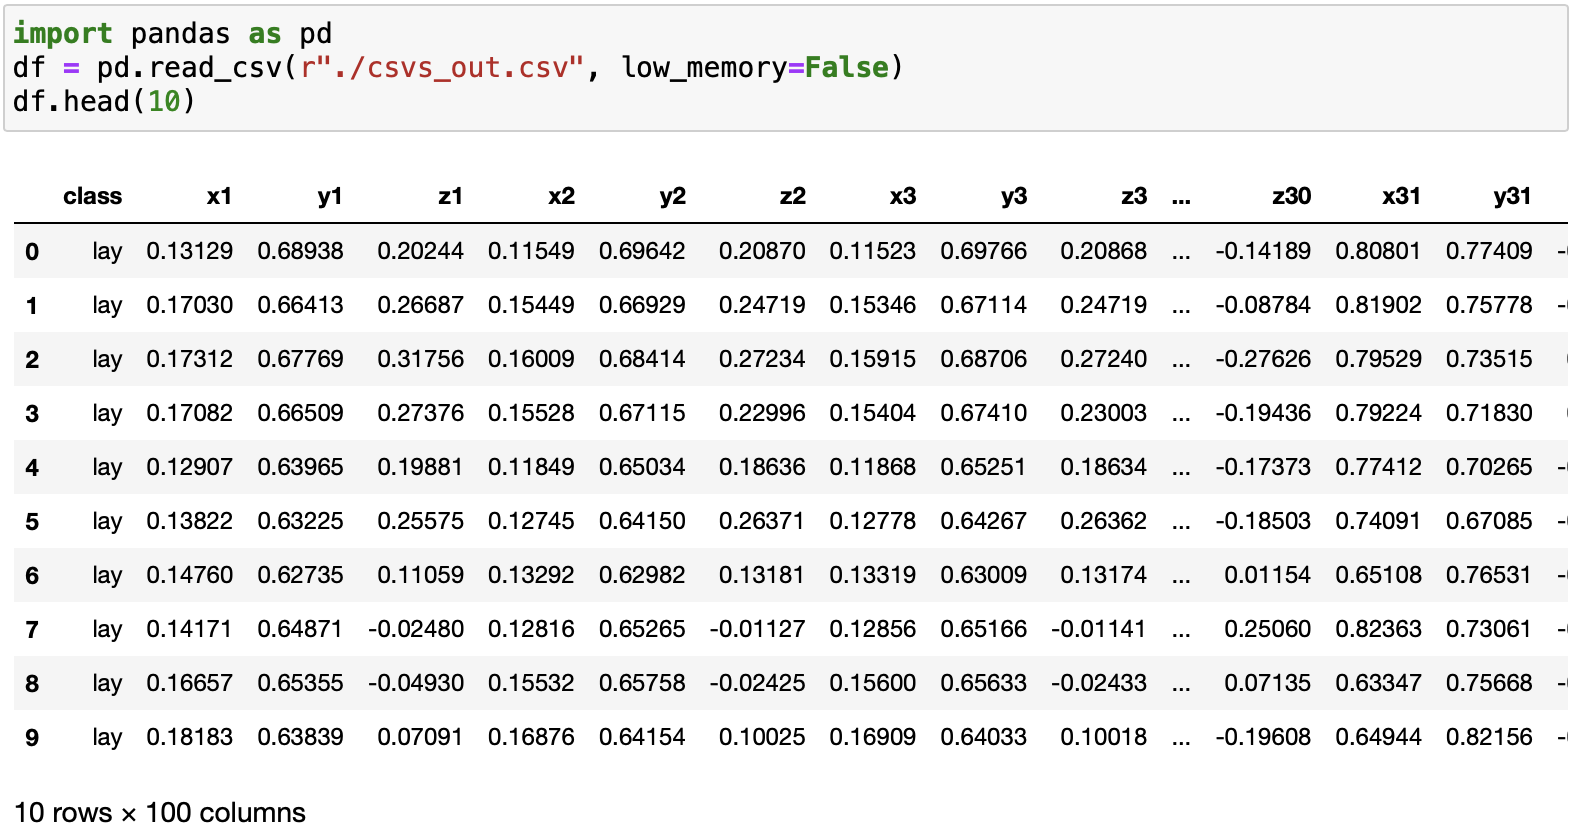
\includegraphics[scale=0.3]{images/csv.png}\end{figure}    
            \item{\large{mediapipe.ipynb}}\\
            The second is mediapipe notebook. It trains the data received and uses the prediction of poses in real-time. There are mainly four parts of this code. \\
            \begin{itemize}
                \item{\large{Installations and initialization: By importing all the modules and libraries needed to run the code, it creates the fundamental environment. }}\\
                \item{\large{Train custom model using scikit learn: Using the CSV file that is obtained through running the above code, it trains the dataset by nominating the target value as a class.}}\\
                \item{\large{Evaluate the model: Then it checks the accuracy of the prediction using scikit learn metrics. }}\\
                \item{\large{Make detections with model: Lastly, using opencv, the code can trigger the camera and turns on the webcam. However, in order to combine with the server side, the photo input is given instead of the real-time base. It then draws landmarks above the human body and face. The accuracy of the current prediction is also shown. The webcam can be shut down by pressing control + q. This is the photo of the webcam predicting standing, sitting, and lying. }}\\
            \end{itemize}
        \end{enumerate}
        \item{\large{Location of Source Code}}\\
        /homealone\_integrate/homeAlone\_AI\\
        \item{\large{Library}}\\
        \begin{enumerate}[label=\roman*.]
            \item{\large{MediaPipe}}\\
            Media Pipe is an Artificial Intelligence (AI) library/framework provided by Google in a single pipeline format so that users can easily utilize an AI function. Since AI model development and training using numerous datasets are also offered in a completed state, vision AI functions can be used like a library where users can simply call it when needed. In addition to face recognition, various vision AI functions such as pose recognition are provided. Among them, Home Alone service was built using pose.\\
            MediaPipe Pose is a Machine Learning(ML) solution for detecting body poses with high-fidelity. It infers 33 landmarks from the face and the body in RGB video frames using BlazePose. \\
            \item{\large{Pipeline}}\\
            Below is the pipeline for MediaPipe. [4]\\
            \begin{figure}[H]\centering 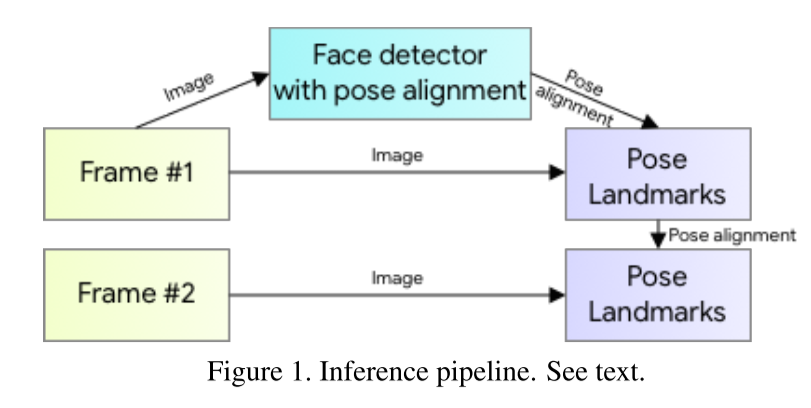
\includegraphics[scale=0.4]{images/pipeline.png}\end{figure} 
            The pipeline consists of a lightweight body pose detector and a pose tracker. The tracker predicts keypoint coordinates, the presence of people, and the ROI of the current frame. If the tracker determines that there is no person, it then reruns the detector in the next frame. The standard of the detector is set as the face because the face has the advantage of having a clear feature and a relatively small deviation. After that, BlazeFace was used to predict additional alignment parameters such as the median coordinates value of a person's pelvis, the size of a circle including a person, and the gradient of a person.\\
            \item{\large{Pose Landmark }}\\
            The current standard for the human pose is a COCO topology, consisting of 17 landmarks across the body, arms, legs, and face. However, COCO key points are confined to ankle and wrist points and therefore lack scale and directional information about hands and feet, revealing limitations when applied to applications such as fitness and dance. On the other hand, BlazePose presents a new topology with 33 pose landmarks. Unlike OpenPose and Kinect topologies, it boasts a fairly fast speed and accuracy to estimate ROI, size, and location using the minimum number of key points of the face, hand, and foot.\\
            The landmark model in MediaPipe Pose uses BlazePose topology. Thus, it predicts the pose with 33 landmarks just like below: [5]
            \begin{figure}[H]\centering 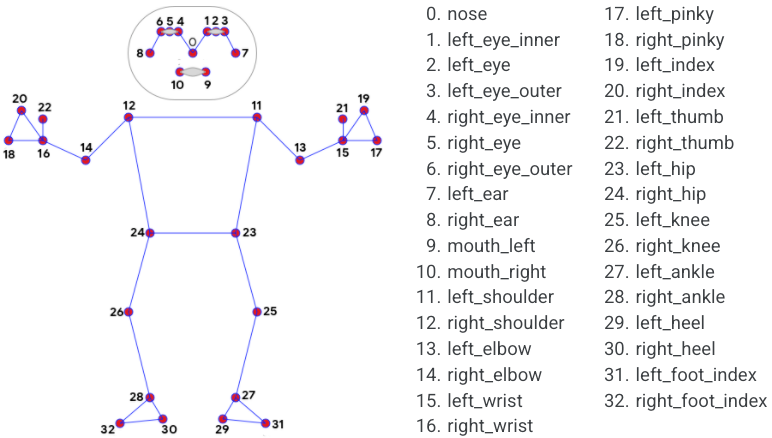
\includegraphics[scale=0.3]{images/pose.png}\end{figure} 
        \end{enumerate}
        \item{\large{Scikit-Learn}}\\ 
        A total of four models were used to predict and classify which class the data belongs to. \\
        \begin{enumerate}[label=\roman*.]
            \item{\large{train\_test\_split}}\\ 
            The train set (learning data set) and test set (validation set) can be easily separated by utilizing the 'train\_test\_split' module in the model\_selection package of the scikit-learn. When dividing the dataset, with the test\_size option, the ratio of Train and Test can be set, and the result can be fixed at every execution time by specifying a seed value with random\_state. Output appears in four forms: X\_train, X\_test, y\_train, and y\_test.\\
            \begin{itemize}
                \item X\_train: Feature part of training data set
                \item X\_test: Feature part of the test data set
                \item y\_train: The label portion of the training data set
                \item y\_test: the label portion of the test data set \\
            \end{itemize}
            By default, the feature part is returned as a data frame, and the label part is returned as a data type in Series. In mediapipe.ipynb, the label will be the class name, that is, stand, sit, and lay. \\
            \item{\large{make\_pipeline}}\\ 
            The pipeline connects the process from data preprocessing to training as one. If the pipeline is not used, the variable selection process is coded, the selected variable is re-standardized, and the model is trained with it. However, by using make\_pipeline, processing the existing process at once is enabled. \\
            \item{\large{LogisticRegression}}\\ 
            Logistic regression is a supervised learning algorithm that uses regression to predict the probability that data belongs to a category either 0 or 1 and determine the category according to its probability. In logistic regression, the following steps are taken to predict the probability that the data belongs to a specific category. \\
            The coefficient and intercept of all features are initialized to zero. Log-odds is obtained by multiplying the value of each attribute by a coefficient. Add log-odds to the sigmoid function to find the probability of the range [0,1]. The Sigmoid function allows the probability to be curved from 0 to 1. \\
            \item{\large{RidgeClassifier}}\\ 
            Overfitting can occur when using the basic linear model. When overfitted, a graph that fits the data so well and therefore extremely rises and falls is created. The coefficient value of linear regression becomes very large too. In order to prevent such a large variance, ridge regression is an algorithm with a penalty if the coefficient itself is large. \\
            \item{\large{RandomForestClassifier}}\\ 
            The ensemble methods combine various learning algorithms and train for machine learning. It not only complements the prediction power but also compensates for shortcomings coming from mere algorithm usage. Ensemble methods include bagging, boosting, and stacking. \\
            Bagging is an algorithm that creates multiple classifiers with the same algorithm. A representative algorithm of bagging is Random Forest.\\
            The decision tree algorithm is classified according to data. Hence, not only did overfitting occur frequently, but when a specific feature called tree correlation influenced the classification a lot, most of the results appeared to be similar to one another.\\
            To improve this, Random Forest is designed with an ensemble method. Random forest is an algorithm based on a decision tree. It is trained by multiple decision tree classifiers based on bagging and makes predictive decisions through voting. Since the random forest is split by bootstrapping, its sample is overlapped.\\
            \item{\large{GradientBoostingClassifier}}\\ 
            Gradient boosting combines several decision trees to create a powerful model. Unlike Random Forest, trees are sequentially generated by reducing the error of the previous tree through learning\_rate, so there is no randomness. In addition, the depth of individual trees is made to be shallow, and the trees with reduced errors are continuously connected.\\
        \end{enumerate}
        \item{\large{OpenCV}}\\ 
        OpenCV is an abbreviation for the Open Source Computer Vision Library. It is a programming library for real-time computer vision. OpenCV is designed with a focus on computational efficiency and real-time applications. Therefore, it is possible to create an application that can be processed in real-time even when coding using the API provided by OpenCV. In other words, high-quality commercial programs can be created without taking care of optimization or algorithms. \\
        In order to prevent invading the privacy issues of the kid, when taking the video, the whole image is blurred by using cv2.GaussianBlur() function. The Gaussian filter mask matrix has a relatively large value at the center, and as it goes to the side, the matrix element value has a value close to 0. Performing a mask operation using such a filter mask is equivalent to obtaining a weighted average by giving a large weight near the pixel to be filtered and a small weight to the periphery far from the pixel to be filtered. That is, the Gaussian filter mask serves as a weight matrix for obtaining a weighted average. \\
        Using the cv2.imread function, the photo is displayed on the monitor. A rectangle is drawn using the cv2.rectangle() function. In addition, after receiving the photo, through cv2.putText(), the desired phrase is shown on the monitor. \\
        \item{\large{Other Modules}}\\ 
        \begin{enumerate}[label=\roman*.]
            \item{\large{OS}}\\ 
            The os module stands for Operating System and allows Python to perform various functions provided by the operating system. By using os.listdir() method, receiving a list of all files and directories in the specific directory was possible. Moreover, the path and filename were combined through os.path.join(). OS module was necessary when creating a single CSV file.\\
            \item{\large{CSV}}\\ 
            CSV is an abbreviation for comma-separated values, and a CSV file is a text file format in which columns of each line are separated by commas. To write a CSV file, open the .csv file in write mode and insert the file object into the csv.writer(). CSV writer adds a line of list data through a method called writerow(). \\
            \item{\large{Pickle}}\\ 
            Pickle allows to save non-text data types as files. pickle.dump() saves the Python object to a file. picke.load() retrieves the pickle file (.pickle extension) stored on the computer as an object within the Python. \\
            \item{\large{NumPy}}\\ 
            NumPy is an external library of Python. When implementing deep learning, this library simplifies the complex calculations of many arrays and row. Using np.array, array is made with landmarks data and using np.argmax, the index of the highest value in a given NumPy array is returned. \\
            \item{\large{Pandas}}\\ 
            Pandas is a Python software library for data manipulation and analysis. In the machine learning code written, an external CSV file was retrieved through the read\_csv() function and stored as a data frame. After that, a new data frame was created using a class constructor named pd.DataFrame(). \\
        \end{enumerate}
    \end{enumerate}
    \item {\large{Module 4: machine learning - 2}} \\
    \begin{center}\large{Face Recognition}\\\end{center} 
    \begin{enumerate}[label=\alph*.]
        \item{\large{Purpose}}\\
        HomeAlone provides customized services for every kid. The LG’s robot cleaner first takes five photos one after another and figures out who that is. It will start operating only when the specific person is detected. For instance, if someone else rather than the person in the uploaded photo, the robot cleaner will simply ignore the data. In order to recognize the image of the person, a machine learning code is required. \\
        \item{\large{Dataset}}\\
        Inside an image folder, one photo of the kid’s image is required. Only one person should be clearly detected in the photo. \\
        \item{\large{Functionality and Code Explanation}}\\
        Face recognition is the process of solving a series of related problems. Modern facial recognition pipelines consist of four stages: detection, alignment, representation, and verification.\\
        The code can be divided into two parts; add\_known\_face and name\_labeling. \\
        \begin{enumerate}[label=\roman*.]
            \item{\large{add\_known\_face}}\\
            This function is for saving the input photo’s data with the name. It is done by using face\_recognition library which will be explained in this document. \\
            \item{\large{name\_labeling}}\\
            It is a function that finds faces, encodes them, compares them, and outputs them. To briefly describe it, finding the face in the image and encoding the face in the detected area is done through this function. Compare the encoding values of the faces found in this way to the known\_face\_encodings list repeatedly that have been registered.\\
            The ‘verified’ variable contains either True or False. It is initially set to False but when it finds the person who is already added to the known face in the photo, it changes to True. \\
        \end{enumerate}
        \item{\large{Location of Source Code}}\\
        /homealone\_integrate/homeAlone\_AI\\
        \item{\large{Library}}\\
        \begin{enumerate}[label=\roman*.]
            \item{\large{face\_recognition}}\\
            Face\_recognition, a python package wraps dlib’s face recognition functions into the simplification version of API. \\
            \begin{itemize}
                \item load\_image\_file: load\_image\_file() function allows to load the image in the format of a numpy array.\\
                \item face\_locations: It returns a 2d array of bounding boxes of human faces in an image. The Convolutional Neural Network (CNN) face detector is used for running this function. \\
                \item face\_encodings: When the image is received, this function returns the 128-dimension face encoding for every face detected in the photo. \\
                \item face\_distance: When the face\_encodings and face\_to\_compare are given, it compares them to a known face encoding. Then it calculates the euclidean distance for each comparison face. The distance is a criterion for the similarity of the faces. \\
                \item compare\_faces: compare\_faces() functions gets three parameters; known\_face\_encodings, face\_encoding\_to\_check, tolerance). known\_face\_encoding is basically a list of known face encodings while the face\_encoding\_to\_check is a single face encoding to compare against. The tolerance represents the distance between faces to determine whether it matches. The smaller the number gets, the stricter it is. \\
            \end{itemize}
            \item{\large{matplotlib}}\\
            By emptying the array of plt.xticks and yticks, deleting all the markings have proceeded. The plt.title of the image was the ‘input image’ and the ‘detected image’. The image was shown by using plt.show().\\
            plt.subplot is applied so that the input image and the detected image with the face border and the person’s name can appear next to one another. \\
            \item{\large{OpenCV}}\\
            The basic explanation of the OpenCV library is written in the pose detection part. In this code, in order to read the image located in the specific directory, cv2.imread() function is used. The location of the photo should be handed over. Also, rectangle() and putText() functions are used again to draw the face’s border to the input image. \\
            \item{\large{NumPy}}\\
            The basic explanation of the NumPy library is written in the pose detection part. To cut it short, in this code, the function argmin() is used. Opposite from argmax() used in the pose detection code,  this function returns the smallest value in a given Numpy array. \\

        \end{enumerate}
        
    \end{enumerate}
\end{enumerate}

\section{\Large{Use cases}}
\begin{enumerate}[label=\arabic*.]
    \item {\large{Scenario 1}} \\
    The first scenario is when the kid is not at home but should be at home according to the schedule data. \\
    \begin{itemize}
        \begin{figure}[H]\centering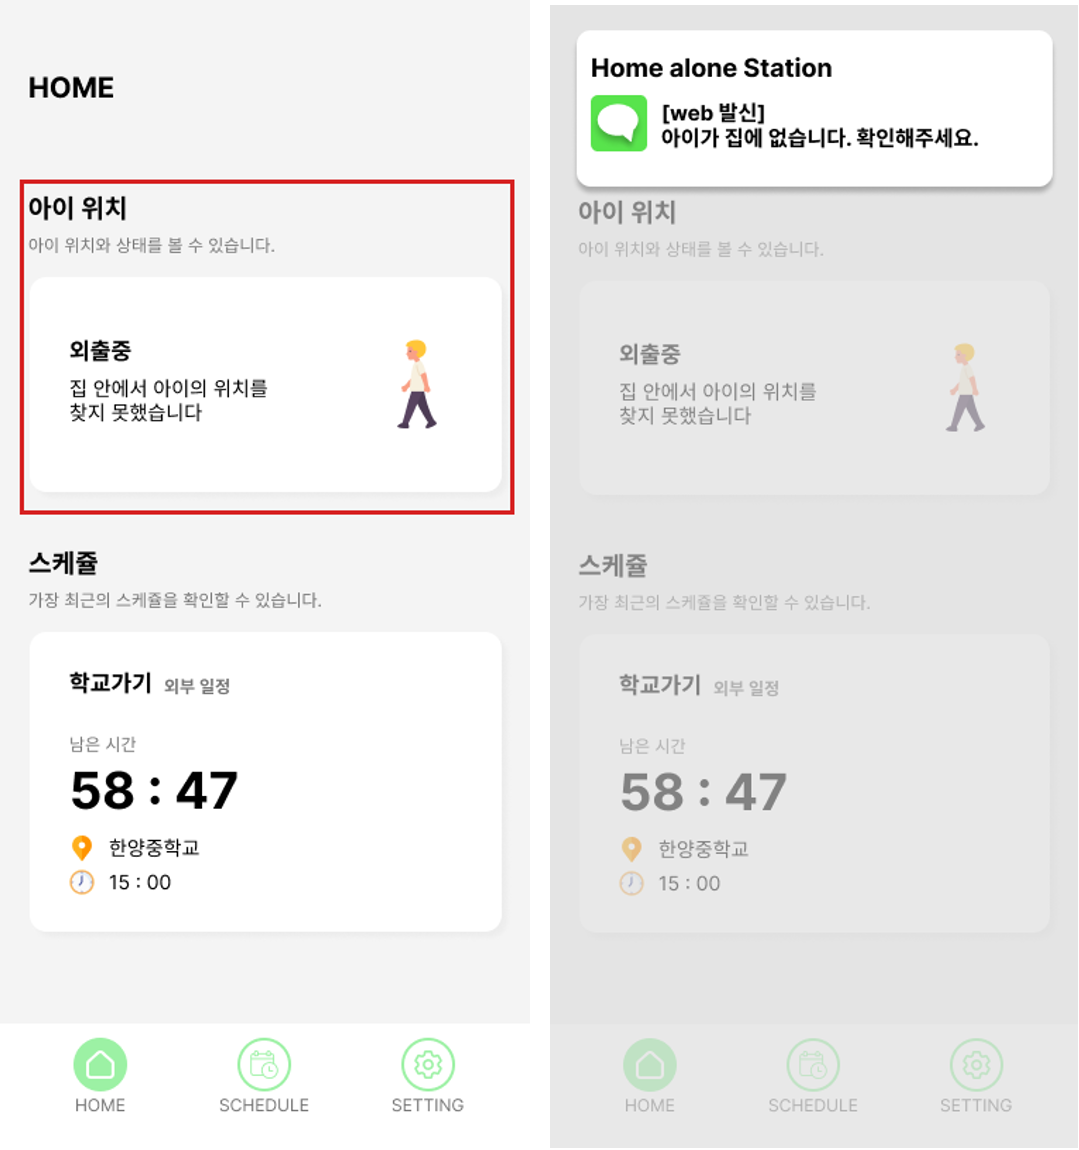
\includegraphics[scale=0.4]{images/scenario1.png}\end{figure} 
        \item App: The app describes the kid’s status as 외출중(Outside), and receives a message from the station server saying “The kid is not at home. Please check.”.\\
        \begin{figure}[H]\centering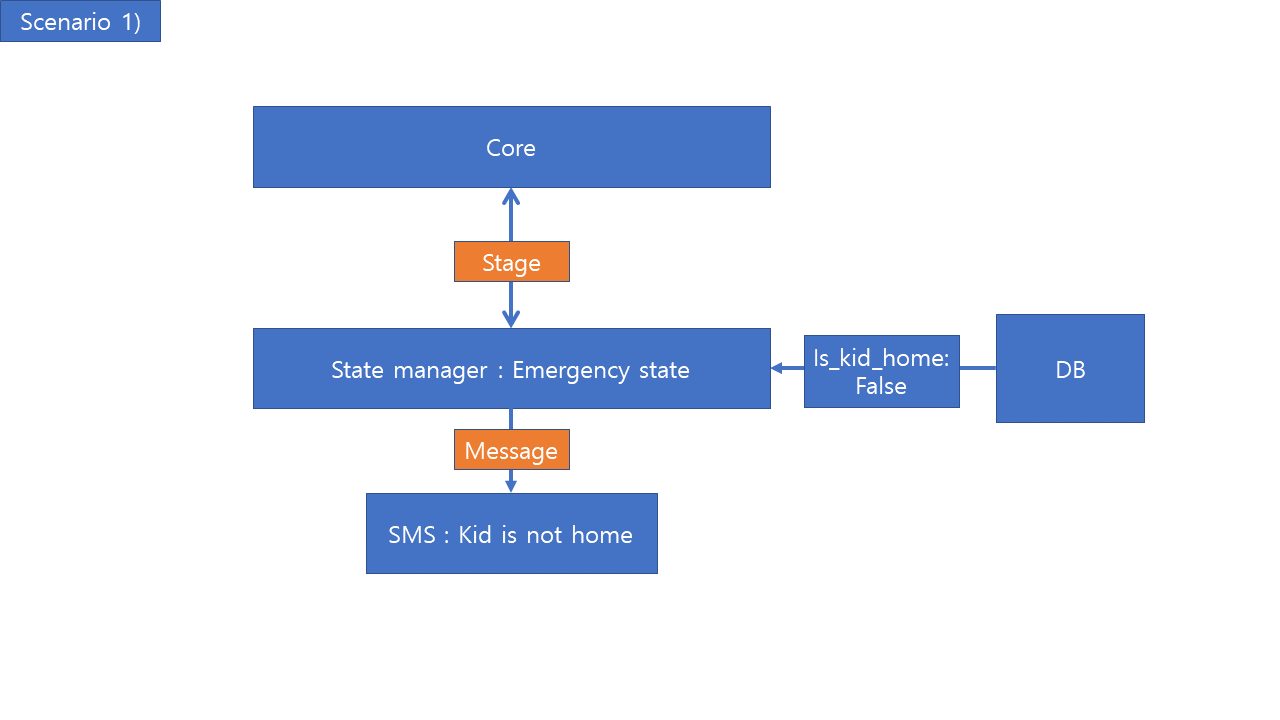
\includegraphics[scale=0.3]{images/s1.png}\end{figure} 
        \item Station: The station receives data from the DB and reacts to the data. \\
    \end{itemize}
    \item {\large{Scenario 2}} \\
    The second scenario is when the kid is late for the upcoming schedule but still laying. \\
    \begin{figure}[H]\centering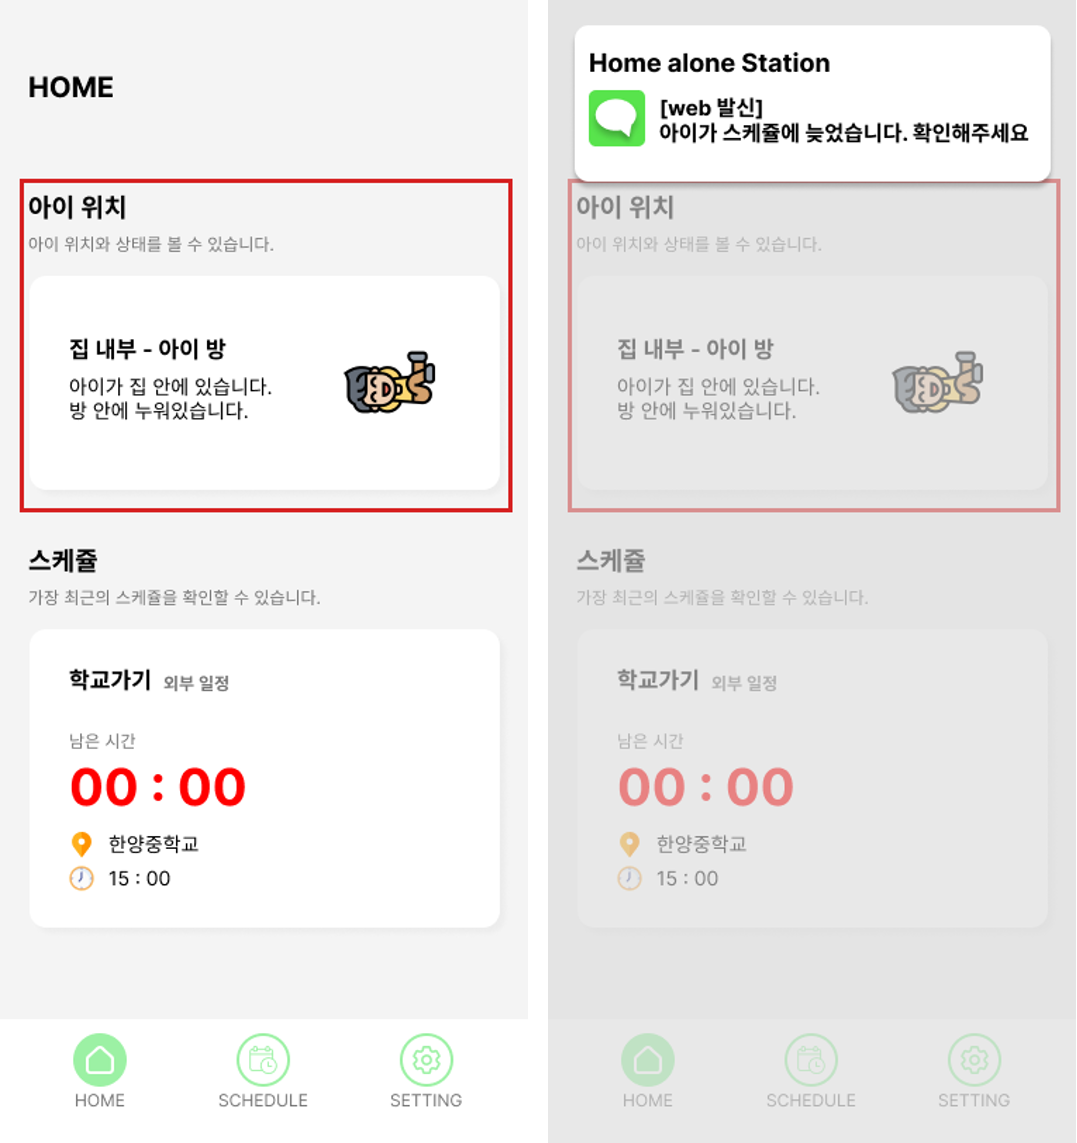
\includegraphics[scale=0.4]{images/scenario2.png}\end{figure} 
    \begin{itemize}
        \item App: The app describes the kid’s status as 집내부 (inside) and 아이 방 (kid-room), and receives a message from the station server saying “The kid is late for the schedule. Please check.”.\\
        \begin{figure}[H]\centering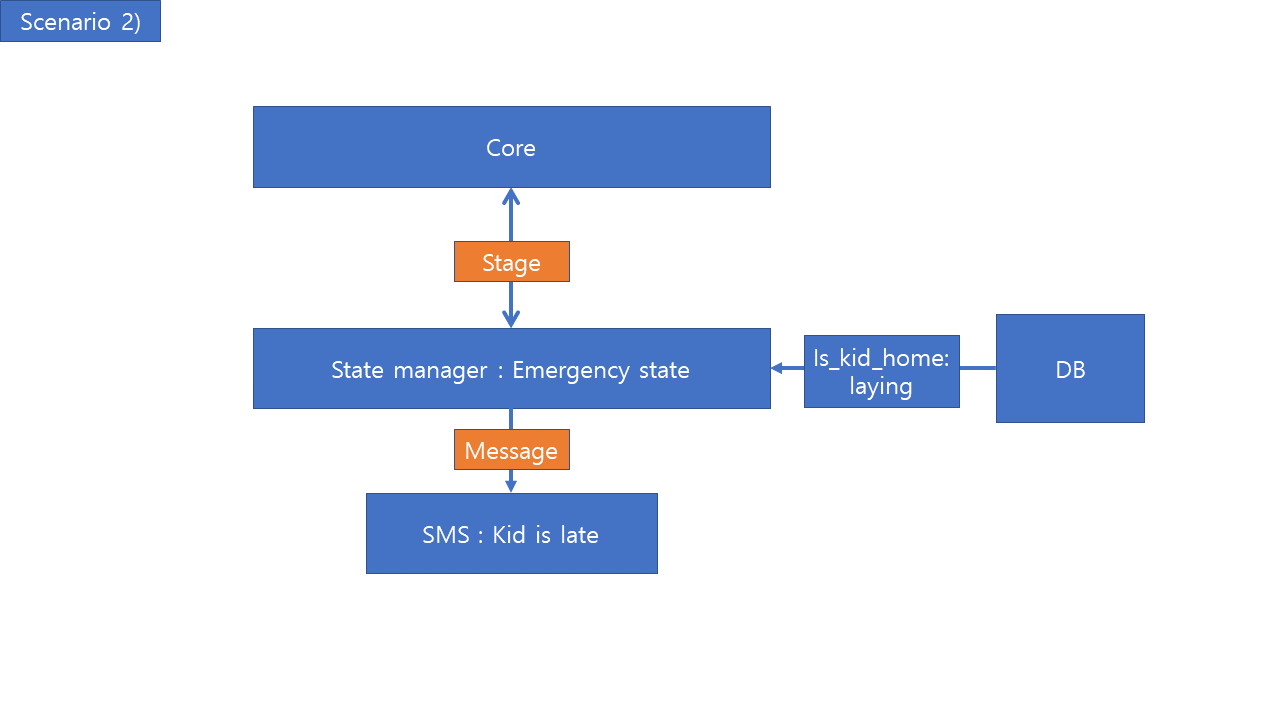
\includegraphics[scale=0.3]{images/s2.png}\end{figure}
        \item Station: The station receives data from the DB and reacts to the data. \\
    \end{itemize}
\end{enumerate}


\end{enumerate}

\begin{thebibliography}{00}
\bibitem{b1} Statistics KOREA Government Official Work Conference, 합계출산율 - 국가지표체계. Retrieved October 21, 2022, from (https://www.index.go.kr/)
\bibitem{b2} Statistics Korea. 저출산의 원인. Retrieved October 21, 2022, from (https://kosis.kr/))
\bibitem{b3} West Seoul Supreme Prosecutor Office. Status of child abduction - Crime analysis. Retrieved October 16, 2022, from (https://www.spo.go.kr/site/westseoul/crimeAnalysis.do)
\bibitem{b4} High Fidelity Pose Tracking with MediaPipe BlazePose and TensorFlow.js - The TensorFlow Blog. Retrieved November 21, 2022, from 
(https://blog.tensorflow.org)
\bibitem{b5} Pose - mediapipe. Retrieved November 21, 2022, from 
(https://google.github.io/mediapipe/solutions/pose.html)
\end{thebibliography}
\end{document}